
%----------------------------------------------------------------------------------------
%	PACKAGES AND OTHER DOCUMENT CONFIGURATIONS
%----------------------------------------------------------------------------------------

\documentclass[12pt]{article}
\usepackage{appendix}
\usepackage[british]{babel}
\usepackage{minted}
\setminted{fontsize=\scriptsize, 
	obeytabs=true,tabsize=2, linenos, frame=lines, framesep=3mm, bgcolor=light-gray, fontsize=\footnotesize}
\usepackage{amsmath}
\usepackage[style=numeric,backend=bibtex]{biblatex}
\addbibresource{references.bib}
\usepackage{graphicx}
\usepackage{float}
\usepackage{url}
\usepackage{booktabs}
\usepackage{hyperref}
\hypersetup{
	colorlinks,
	linkcolor={black},
	citecolor={blue!80!black},
	urlcolor={blue!80!black}
}
\usepackage{blindtext}
\usepackage[table,xcdraw]{xcolor}
\usepackage{listings}
\usepackage{color}
\definecolor{light-gray}{gray}{0.95}
\lstset{
	numbers=left,
	breaklines=true,
	backgroundcolor=\color{light-gray},
	tabsize=2,
	basicstyle=\ttfamily,
}


\usepackage{hyperref}
\hypersetup{linktoc = all}
\renewcommand{\arraystretch}{1.5}	% Increase row space between tables



\begin{document}

	
	\begin{titlepage}
		
		\newcommand{\HRule}{\rule{\linewidth}{0.5mm}} 
		
		\center % Center everything on the page
		
		%----------------------------------------------------------------------------------------
		%	HEADING SECTIONS
		%----------------------------------------------------------------------------------------
		\textsc{\Large MSc Project: Mobile Hairdresser Application}\\[5 cm] 
		
		
		
		
\includegraphics[scale=0.05]{images/logo.png}\\[1 cm]
		
		
		
		
		
		\textsc{\LARGE Joshua Robertson} \\[6 cm]
		
		
		
		
		
		%----------------------------------------------------------------------------------------
		%	TITLE SECTION
		%----------------------------------------------------------------------------------------
		
		
		
		%----------------------------------------------------------------------------------------
		%	AUTHOR SECTION
		%----------------------------------------------------------------------------------------
		
		
		\begin{center}
			
			\textsc\emph{{“A dissertation submitted to the University of Bristol in accordance with the requirements of the degree of Master of Science by advanced study in Computer Science in the Faculty of Engineering."}} \\[1.2 cm]
			
			School of Computer Science, Electrical and Electronic Engineering, and Engineering Maths (SCEEM) \\[1 cm]
			
			
			
		\end{center}
		
		
		
		
		\vfill % Fill the rest of the page with whitespace
		
	\end{titlepage}


	\section*{Executive Summary}

	
	\pagebreak

	\section*{Acknowledgements}
	\pagebreak
	
	\section*{Author's Declaration}

	I declare that the work in this dissertation was carried out in accordance with the 
	requirements of the University’s Regulations and Code of Practice for Taught Programmes 
	and that it has not been submitted for any other academic award.  Except where indicated 
	by specific reference in the text, this work is my own work. Work done in collaboration with, 
	or with the assistance of others, is indicated as such. I have identified all material in this 
	dissertation which is not my own work through appropriate referencing and 
	acknowledgement. Where I have quoted or otherwise incorporated material which is the 
	work of others, I have included the source in the references.  Any views expressed in the 
	dissertation, other than referenced material, are those of the author. 
	\\
	\\
	SIGNED: Joshua Robertson DATE: 14.09.2021 
	
	\pagebreak
	
	{
		\hypersetup{linkcolor=black}
		\tableofcontents
		\pagebreak
	
		\listoffigures
		\pagebreak
	}
	
	\hypersetup{linkcolor={blue!80!black}}
	
	\section{Introduction}


	
	
	The COVID-19 pandemic has had a ubiquitous impact on our lives, from work, to travel, to how we socialise. Some of these changes are temporary, such as mask wearing, but others, such as the adoption of more digital services and flexible homeworking seem likely to be permanent (ADD CITE). 
	Subsequently, the restriction of movement has caused consumers to migrate to online services at an unprecedented rate. With the global home services market expected to grow by almost 20\% per year until 2026 \cite{ray28StatisticsHome2021} there exists a wealth of opportunity for companies to capitalise through digitalising previously physical services. One of these services is hairdressing, which saw a sizeable uptake in demand throughout the pandemic. 
	\\
	
	There already exists a range of applications suited towards providing home haircuts. For example, Shortcut \cite{incShortcutInHomeHaircuts}, TRIM-IT\cite{TRIMITMobileBarbershopsa} and TrimCheck\cite{TrimCheckHomeHaircuts} all provide bookable home haircuts. Despite this, none of the aforementioned applications follow the "uber" model, of allowing for immediate booking and delivery of home haircuts. 
	\\
	
	This application will therefore aim to facilitate this, along with exploring any other market gaps through early research and will aim to achieve this through the following objectives:
	\\
	
	\noindent
	$\bullet$ Conduct research to elucidate any market gaps
	\\
	$\bullet$ Through a user centric design (UCD) methodology plan and prototype the user interface of the application
	\\
	$\bullet$ Create a minimum viable product (MVP) using new product development (NPD) methodologies
	\\
	
	The research aspect of the project will aim to analyse the strength and weaknesses of existing applications within the field, therefore exposing any market gaps that may be present. 
	
	For the implementation of the application, a heavy focus on the end user was taken through using a UCD methodology, along with NPD, which refers to the  entirety of processes leading to bringing a product to market and encompasses several steps as seen in figure \ref{fig:npd} below and discussed throughout the proceeding sections.
	\newline
	
	\begin{figure}[H]
		\centering
		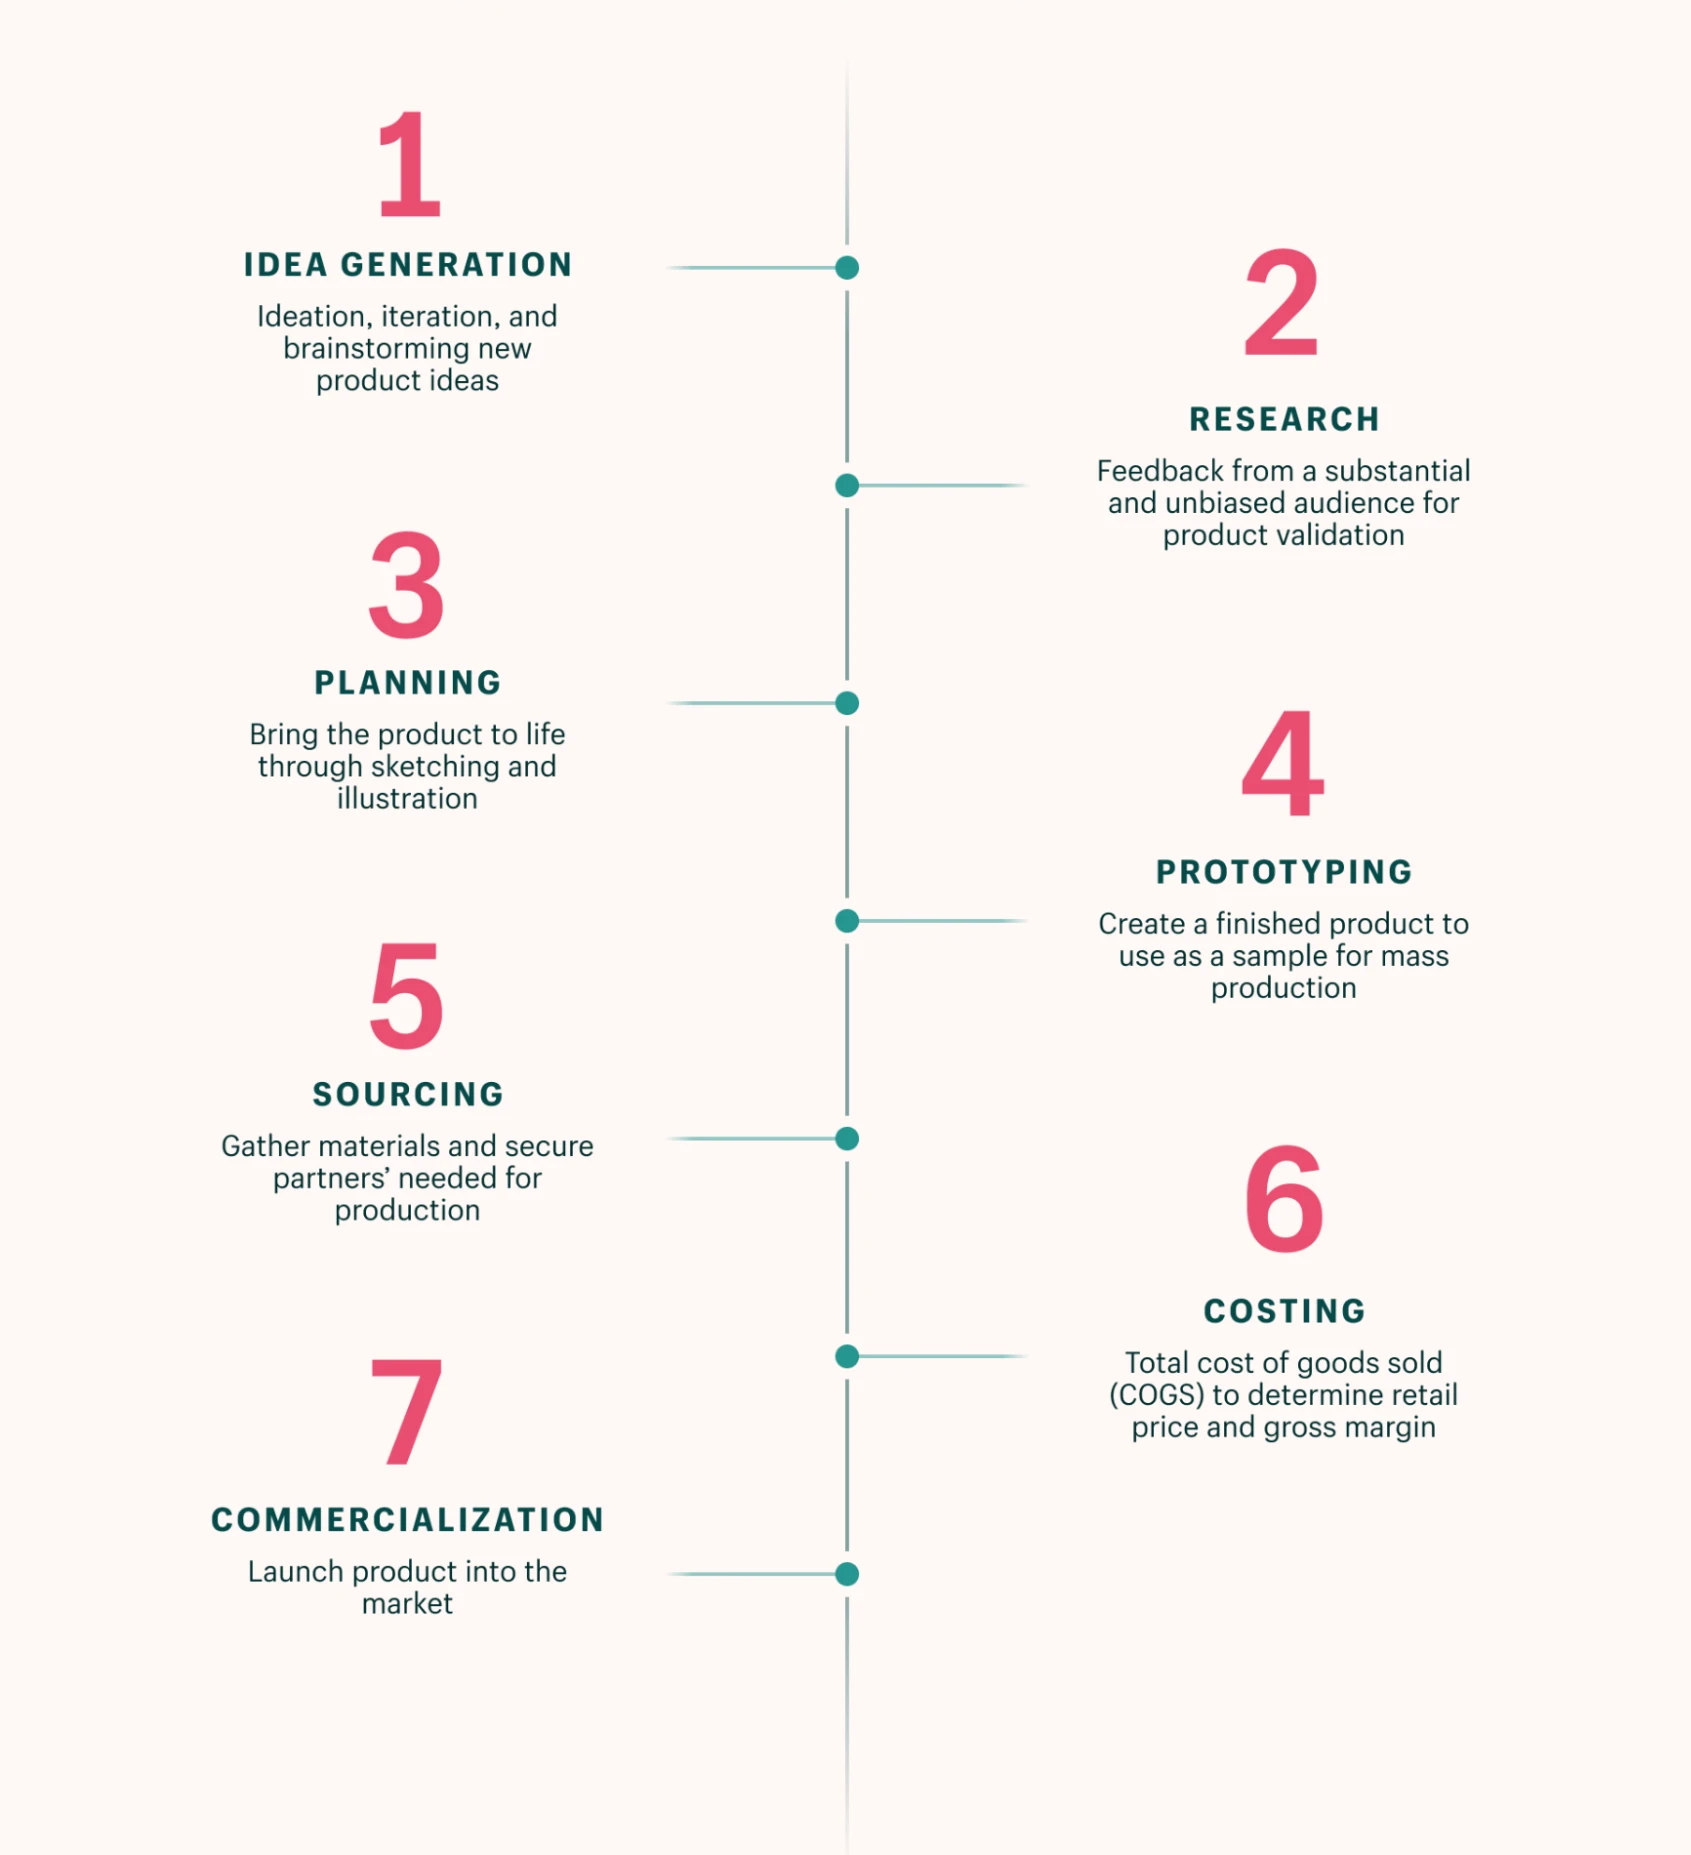
\includegraphics[scale=0.15]{images/npd.png}
		\caption{The 7 Steps of New Product Development}
		\label{fig:npd} \cite{shopifyWhatProductDevelopment}
	\end{figure}
	
	
	\subsection{Ideation and Concept}
	The first stage of NPD starts with conceptualisation of a product idea. For the application the initial concept came from an external partner, who proposed a mobile hairdresser application to capitalise on the increased need for home delivery services. This was further defined during several meetings carried out in the initial stages of the project.
	\\
	
	\subsection{Project Management}

	The project management for the application focused on two key aspects; a clear vision and scope, including a detailed project plan; and an execution phase, which utilized an agile methodology.
	
	\subsubsection{Vision and Scope}
	The end goal of the project was as a springboard to create a fully functional and profitable barber delivery application.
	
	The scope of the project was..
	
	\subsubsection{Agile Methodology}
	To carry out the project, an agile methodology was utilised, which allowed for short, iterative cycles of production, providing value in the form of quick creation and constant revision. Taking on an agile methodology also served the project well in the sense that there was a strong focus on prioritising value over comprehensive documentation and lengthy processes. 
	
	Although this approach is more commonly relevant to a team of developers, approaching the project management in this way allowed for a stringent and well defined timeline to be used, aiding in project delivery and outcome. This involved several key stages.
	Firstly, individual 'epics' were defined, which included:
	\\
	$\bullet$ Define the Scope and Market Research
	\\
	$\bullet$ Design and Architect the Application
	\\
	$\bullet$ Setup and Create The Backend
	\\
	$\bullet$ Write the Dissertation
	\\
	
	These were then used to create 'stories' which were further split into individual tasks placed into a timeline and carried out in . For this, the project management tool monday.com \cite{MondayHome2021} was used, which can be seen in figure \ref{fig:monday.com}. Using Monday.com allowed for a timeline to be easily created, along with updating the status of each story when relevant to follow the completion of the project. In this way, a change management approach (ADD CITE) could be carried out, in which the project could easily be updated and reflected in the tasks. This was especially important as both agile methodology and the UCD rely on constant feedback from the end user which informs the project.
	
	\begin{figure}[H]
		\centering
		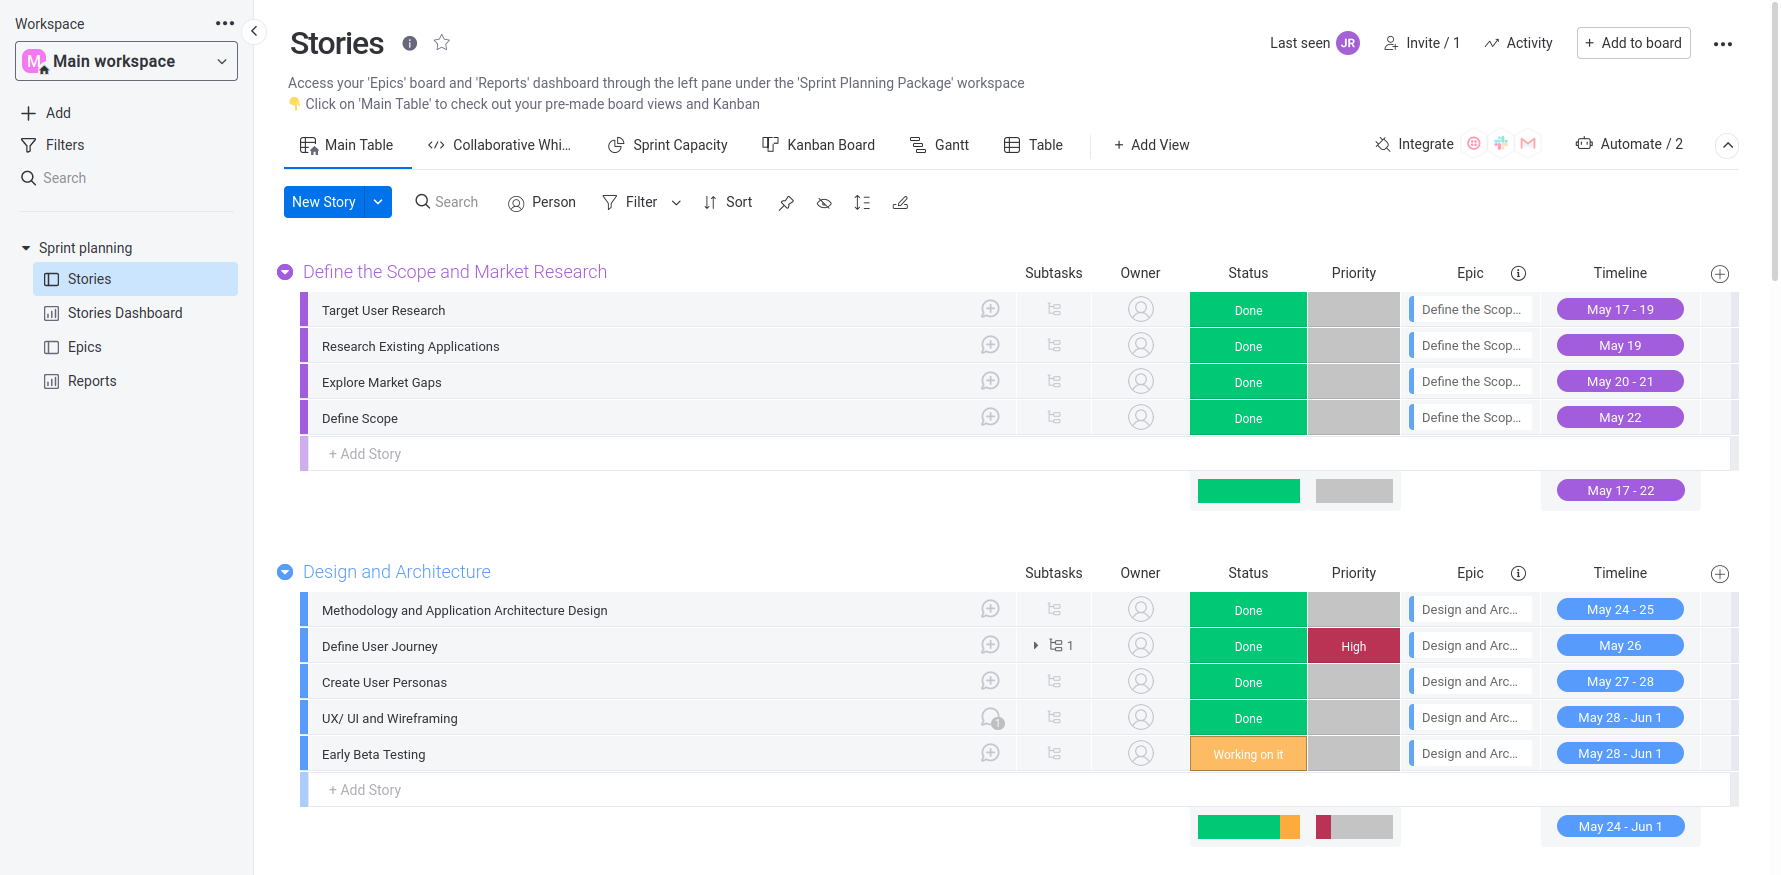
\includegraphics[scale=0.25]{images/monday.png}
		\caption{Screenshot of Monday.com Displaying the Project Stories}
		\label{fig:monday.com}
		\cite{MondayHome2021}
	\end{figure}

	Finally, using the created timeline, a gantt chart was implemented, which gave an overarching view of the project, with tasks performed represented along the vertical axis and the timeline represented along the horizontal axis. This can be found in the appendix (ADD CITE).
	
	\subsection{Research and Market Analysis}
	\label{market-analysis}
	In order to gauge whether there is a market for the proposed analysis, a survey was carried out in which users were asked about whether they could see themselves using the application features, among other things. The full survey can be found within the appendix (ADD CITE)
	
	\subsubsection{Existing Applications}
	As previously discusses there exists a variety of similar applications, for which the most prominent will be discussed below, along with the salient and limiting features of each.
	\\
	TODO: finish this section
	
	\noindent
	\underline{Shortcut}
	\\
	Shortcut is a US based application..
	One of the defining features of the shortcut app is the availability, with the app providing the ability to request a haircut from 8am to as late as midnight capatilising on a previously unventured late night hair cut market.
	
	The application is limited on it's features, with it only having the option to request a Hair Cut only or a Hair Cut and Beard Trim. 
	Another limiting feature of the application is the price. For a single haircut the cost starts at 75\$ (around £54), which is most likely a reflection of high start up costs and is a problem seen in other similar applications, such as uber and lyft that can only be mitigated through losses (\cite{WillRidehailingProfits}).
	\\
	
	\noindent
	\underline{TRIM-IT}
	https://www.bbc.co.uk/news/stories-47711610
	TODO: discuss more here
	\\
	TRIM-IT is a UK based mobile hairdressor application. Their business model is franchise based similar to that seen by Mcdonald's, whereby barbers would invest through a monthly fee and be provided with the tools necessary, such as a mobile barber unit. 
	
	\noindent
	\underline{TrimCheck}
	
	
	\subsubsection{Novelty of the Proposed Application}
	As discussed in the previous sections, there exists a range of applications that are suited towards providing a mobile barber service.
	
	(shortcut)The ability to offer a variety of services not limited to just a haircut or beardtrim.
	
	\subsection{Deciding on a Platform}
	\label{chap:platform}
	\subsubsection{Mobile vs Desktop}
	An important consideration in NPD is determining which platform best suits the project, mobile or desktop. Here, we will discuss the merits and pitfalls of each, before concluding which is most relevant for the project. 
	\\
	
	\noindent
	\underline{Market Share}
	\\
	\noindent
	Consumers are now for the first time viewing web pages on mobile devices at a higher rate than on desktop, at 54.8\%, compared to just 31.16\% in early 2015 \cite{MobilePercentageWebsite2021}. Further to this, over the last year desktop usage has dropped from 46.39\% to 41.36\%, whilst mobile phone usage has increased from 50.88\% to 55.89\%, following on a several year long trend \cite{DesktopVsMobile2021} that reflects a saturated mobile market driving down the cost of phones. However, this analysis is slightly premature due to only being indicative of the world market, whereas the proposed application will only operate within the United Kingdom. When we analyse just the U.K. data (figure \ref{fig:uk-mobile-desktop}) we see that the results are not so conclusive, with only a 0.97\% difference between the two in favour of Desktop. Therefore a decision based entirely on market share is unfavourable and other metrics must be explored.
	
	\begin{figure}[H]
		\centering
		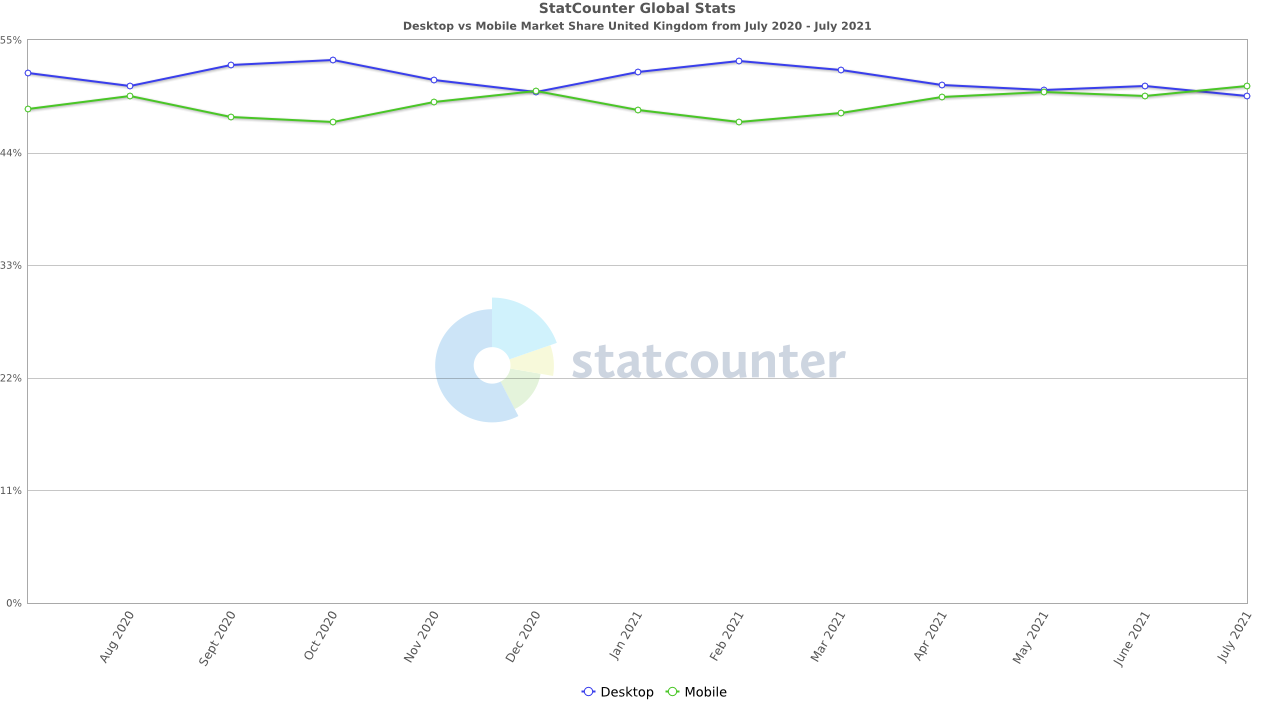
\includegraphics[scale=0.45]{images/GB-mobile-desktop.png}
		\caption{Desktop vs Mobile Market Share in the United Kingdom}
		\label{fig:uk-mobile-desktop}
		\cite{DesktopVsMobile2021a}
	\end{figure}

	\noindent
	\underline{Features and Performance}
	\\
	\noindent
	Another metric to take into consideration is which features are required for the application and how this is reflected in mobile vs desktop applications. One the most pertinent features required is geolocation, which is much more suited to a mobile application due to inbuilt GPS. Another important consideration for the project is speed, for which mobiles perform actions much faster than a website. Finally, as continuation of the project to market is expected, speed of creation is essential, for which an application is better suited.

	
	\subsubsection{Mobile Platform: Android vs iOS}
	An important consideration when creating a mobile application is deciding on which platform to choose. The two largest mobile providers currently are android and apple (iOS). Historically, iOS has dominated the market share, with a 42.02\% market share in January 2011 compared to Androids 12.42\% (figure \ref{fig:ios-android}). Despite this, in recent years android OS has become more popular, even holding a greater share several times over the last few years and currently trails by only around 2\%.
	
	\begin{figure}[H]
		\centering
		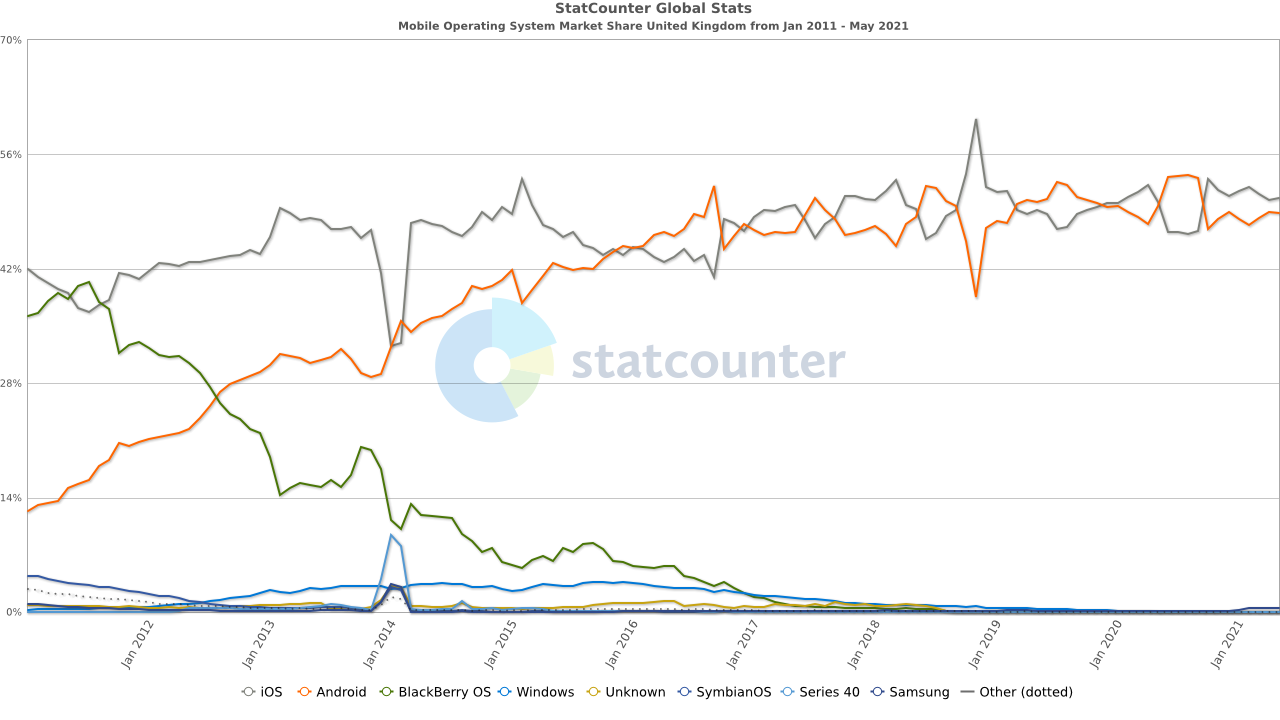
\includegraphics[scale=0.4]{images/ios-android.png}
		\caption{iOS vs Android Market Share Over The Last 10 Years}
		\label{fig:ios-android}
		\cite{AndroidVsIOS2021}
	\end{figure}
	
	With this change has brought with it a push towards frameworks that allow for development across multiple platforms, such as React Native (\cite{ReactNativeLearn}) and Flutter (\cite{FlutterBeautifulNative}). For this reason, it was decided that a cross platform framework would be used, which is further discussed below.
	
	\subsection{Frontend: Programming Language}
	When deciding on the programming software, several metrics were taken into consideration, including cross-platform functionality, speed, speed of development and performance. For this reason, Dart and the corresponding Flutter software development kit (SDK) were chosen for the primary software. Flutter is a cross-platform development kit, meaning that it will natively run on both iOS and android applications created by Google \cite{FlutterBeautifulNative}. Dart is compiled ahead-of-time into native ARM code giving better performance compared to other similar development kits, such as React Native and the user interface  is implemented within a fast, low-level C++ library giving great speed to the application. Dart has also seen a large increase in usage within recent years, jumping up 532\% from 2018 to 2019 \cite{StateOctoverse2019} meaning that there is now an extensible list of third-party plugins available and a large community.
	
	\subsection{Backend: SQL vs noSQL database}
	For the database, it was decided to use Google Firestore (\cite{CloudFirestoreFirebase}), a noSQL database that relies on  nested 'documents' within 'collections'. This was chosen for several reasons. Firstly, as the chosen language 'Dart' is run by Google, using firestore allows for greater integration and congruence with the platform and APIs. Firestore also allows for rapid scalability, along with using Googles excellent cloud platform. The cloud firestore also integrates well with Firebases Authentication service, which is used throughout and discussed extensively in \autoref{chap:implementation}
	
	Another important feature of noSQL databases is the ability to easily modify the internal data in response to changing business requirements, in an interactive way that allows fordo you use relationship data in firebase stackoverflow modification throughout the application lifestyle and therefore easy scaling.
	
	

	
	
	\subsection{The Target User}
	\label{chap:target-user}
	The planned application targets any user who wishes to get a haircut from their home.
	TODO: finish target user section 

	
	
	\subsubsection{User Personas}
	\label{user-personas}
	The creation of user personas representing fictitious, archetypal users is an essential part of application development \cite{PDFPersonasParticipatory} and allows a deep understanding of the target user to be sought and implemented within the features and design of the application \cite{arnowitzChapter15Wireframe2007}. There are, however, some shortcomings to qualitative persona generation, such as validity concerns and user bias \cite{chapmanPersonasNewClothes2005} and although they are addressed by other methods, such as data-driven personas \cite{mcginnDatadrivenPersonaDevelopment2008}, these require a broad user base and therefore we have decided to stick with qualitative methods, which allow for enough brevity and depth for the scope of the project.
	
	Here 4 user personas were created, which are discussed in detail below.
	\newline
	
		\underline{Persona 1 - Sarah Johnson}
		
		Profile: 
		\begin{figure}[H]
			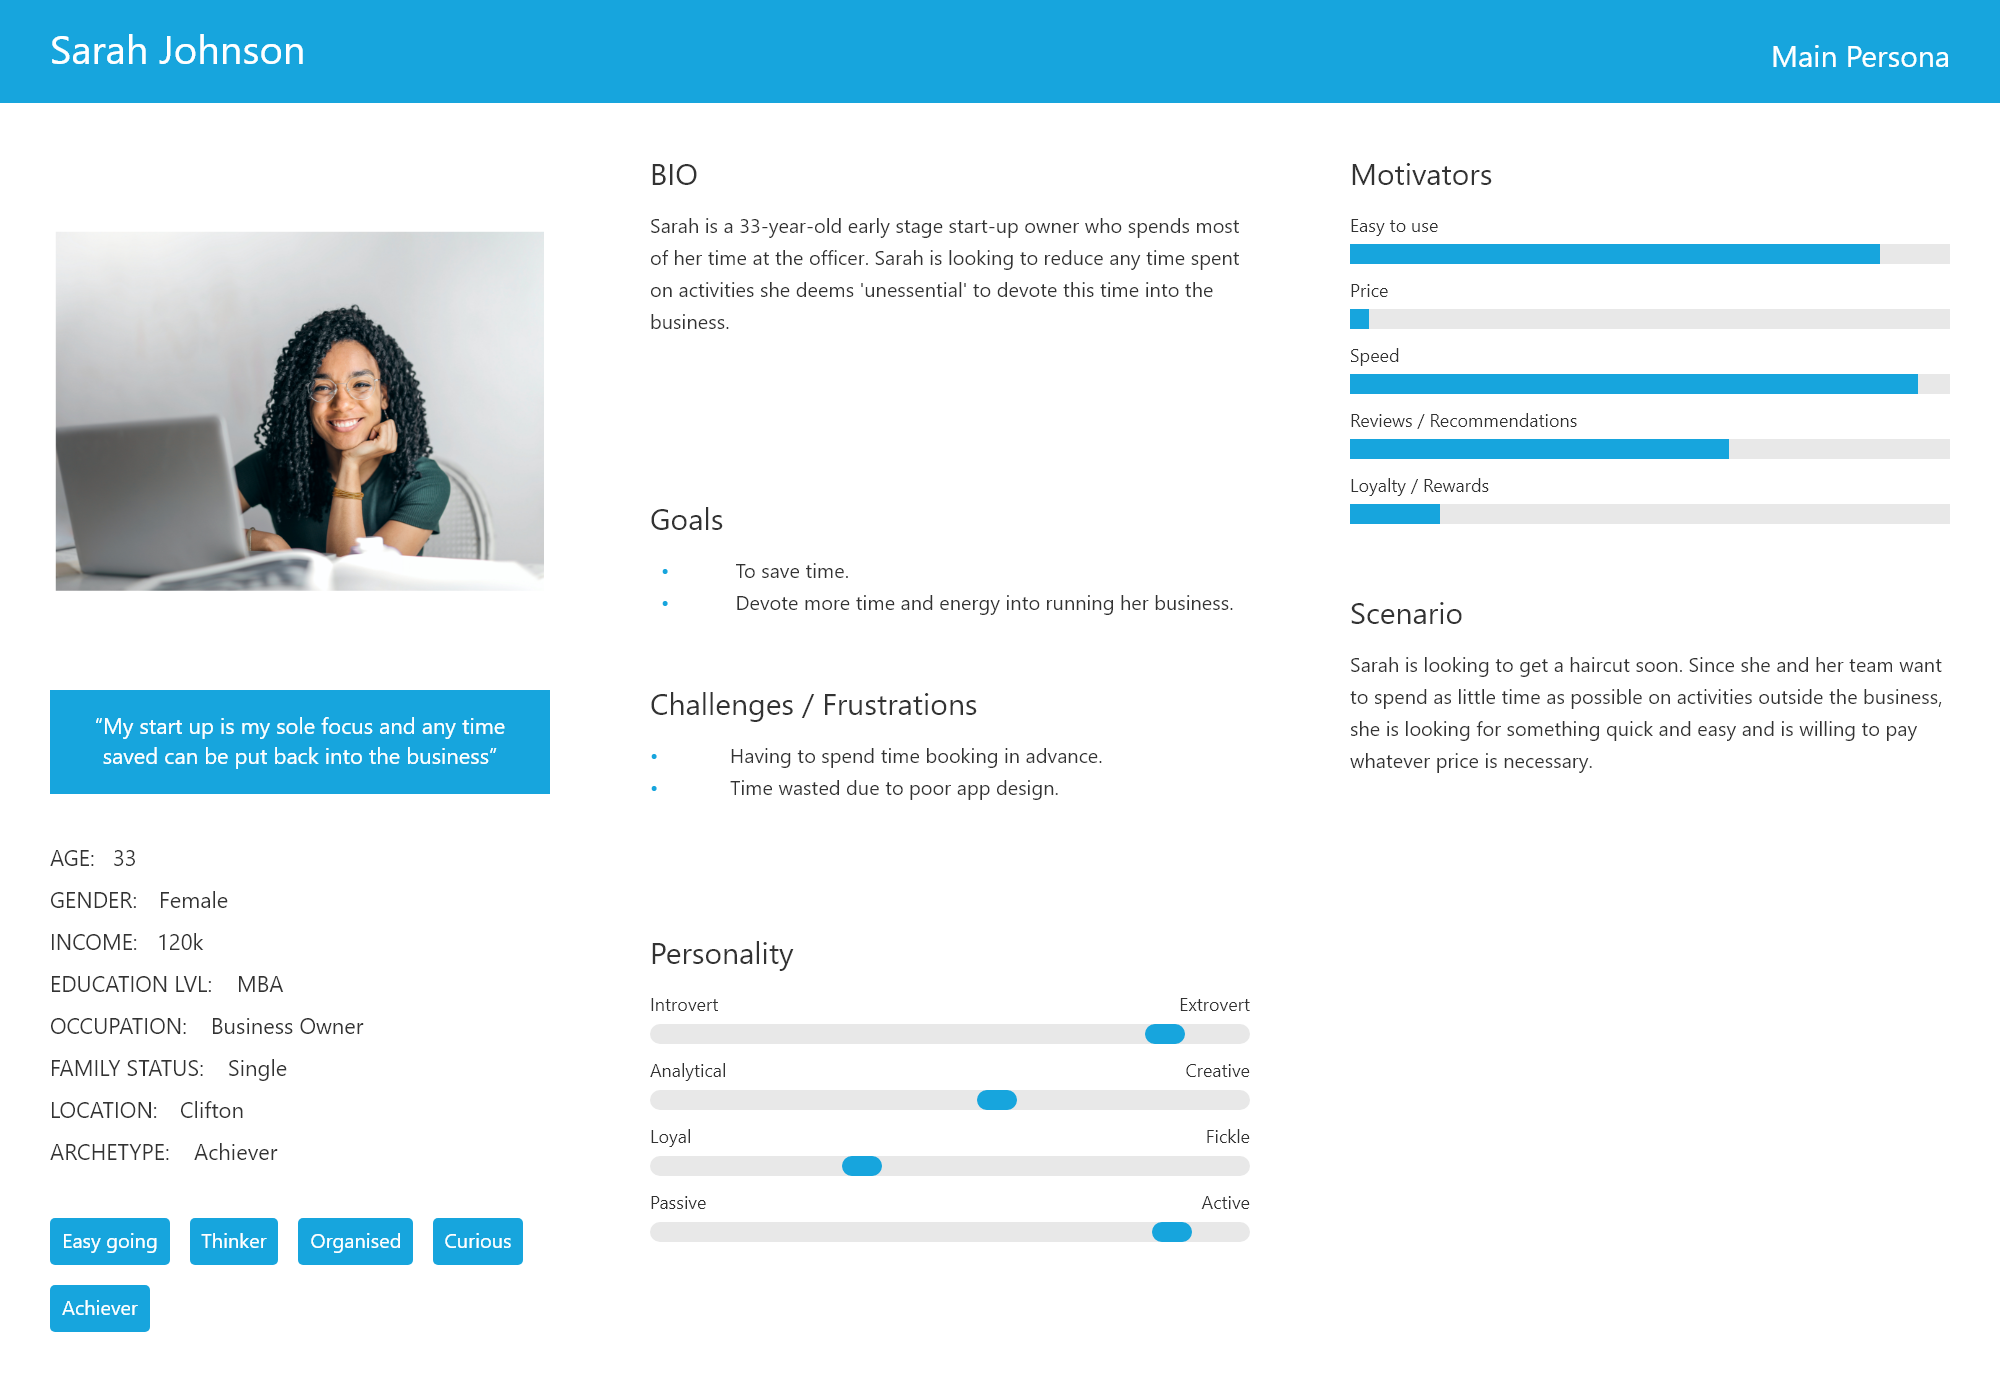
\includegraphics[scale=0.2]{images/persona_1.png}
			\caption{Persona 1}
			\label{fig:persona_1}
		\end{figure}
	

		
		\underline{Persona 2 - Juan Smith}
		
		
		Profile: 
		\begin{figure}[H]			
			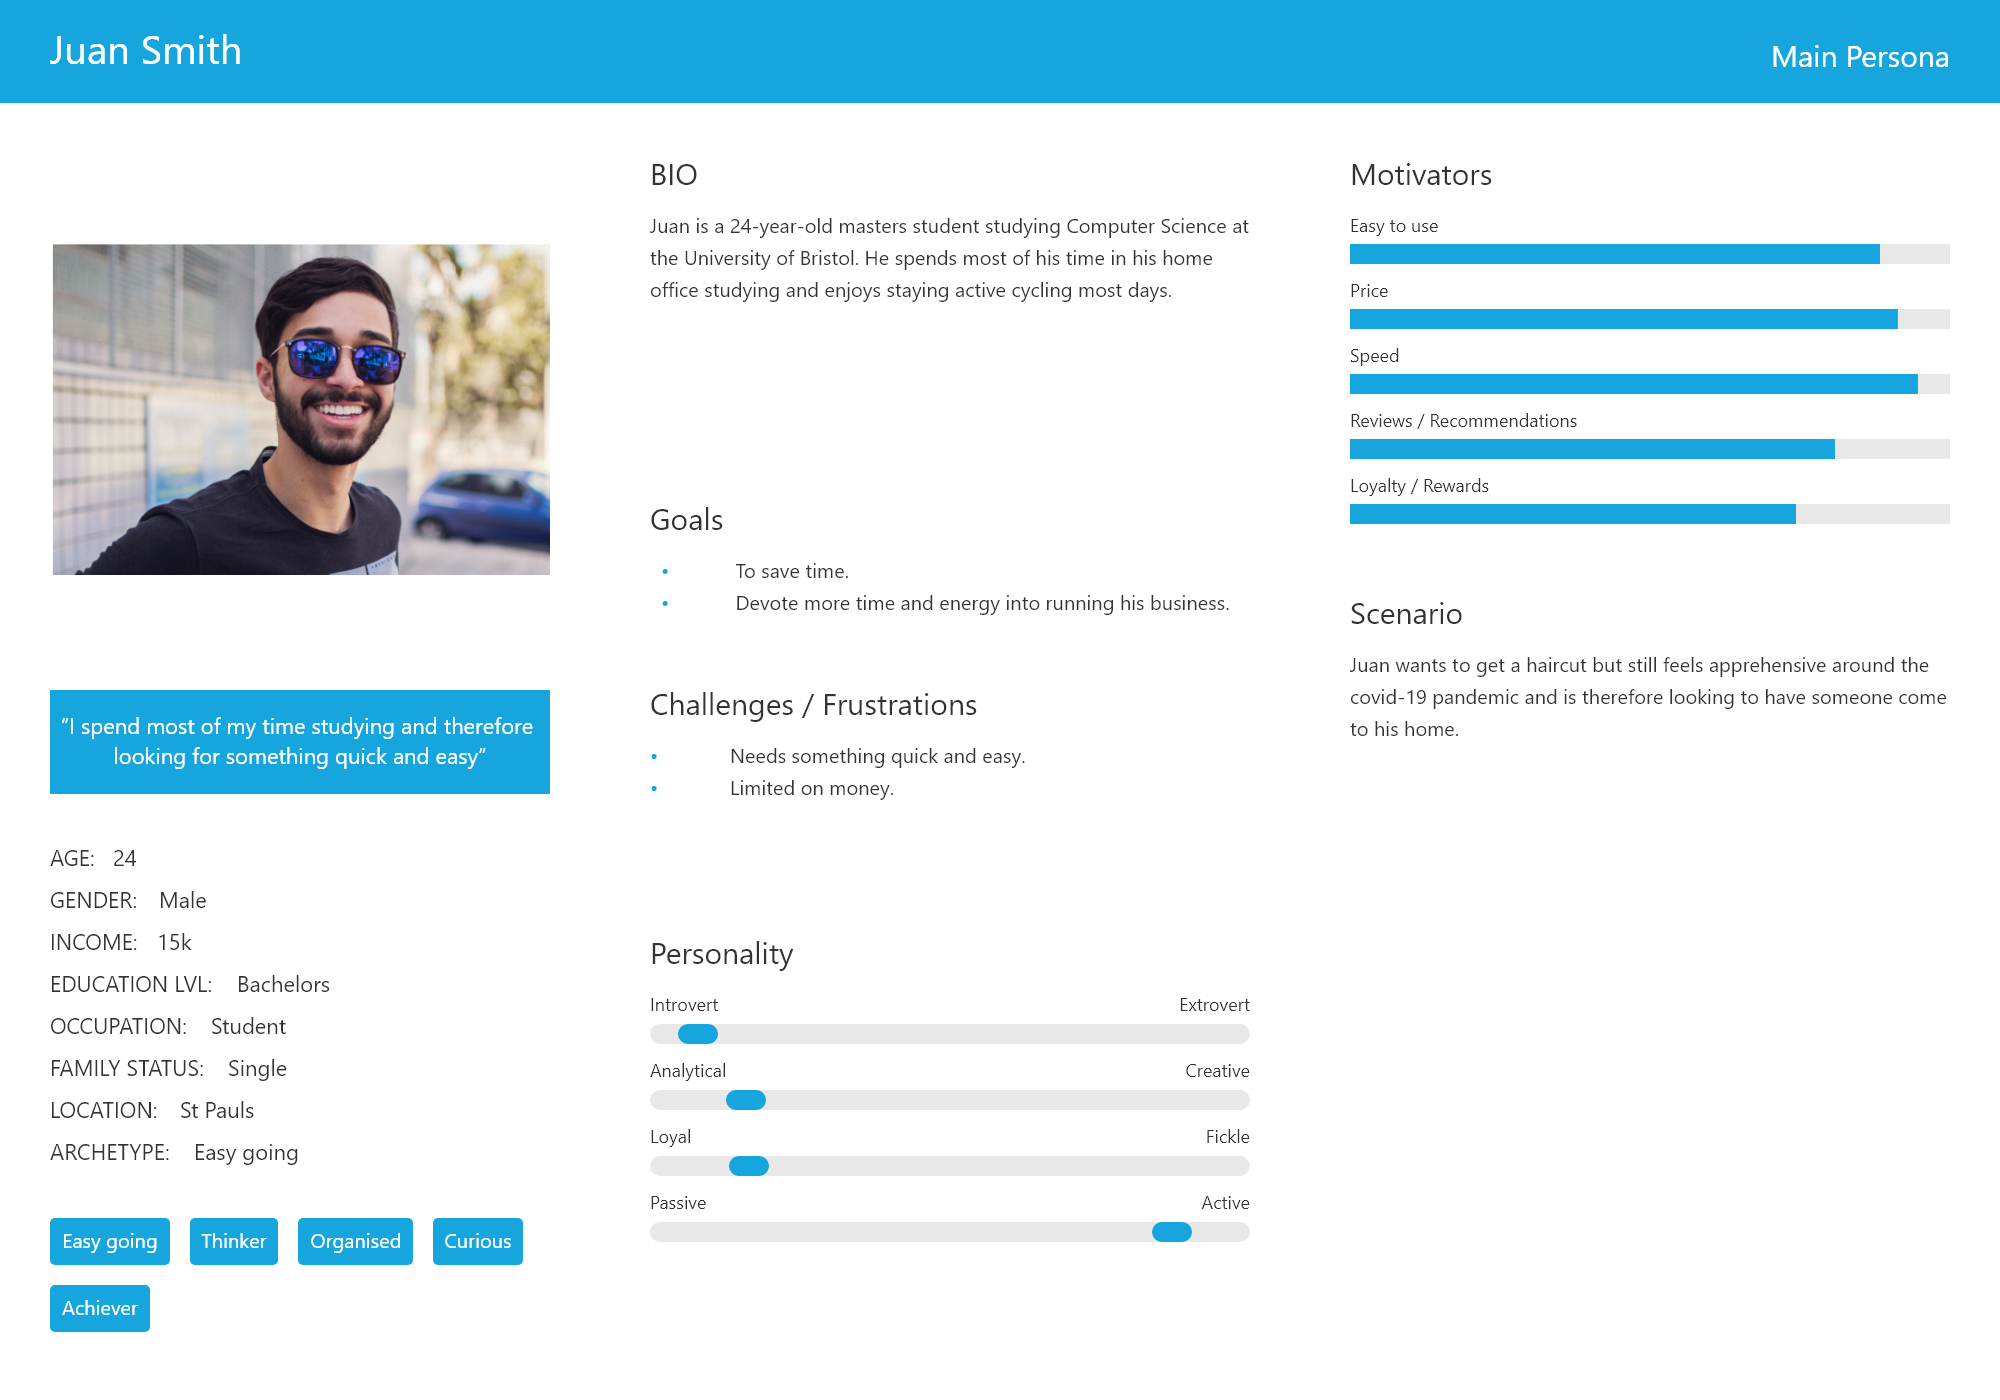
\includegraphics[scale=0.2]{images/persona_2.png}
			\caption{Persona 2}
			\label{fig:persona_2}
		\end{figure}
		
		\underline{Persona 3 - Emily White}
		
		Profile: 
		\begin{figure}[H]			
			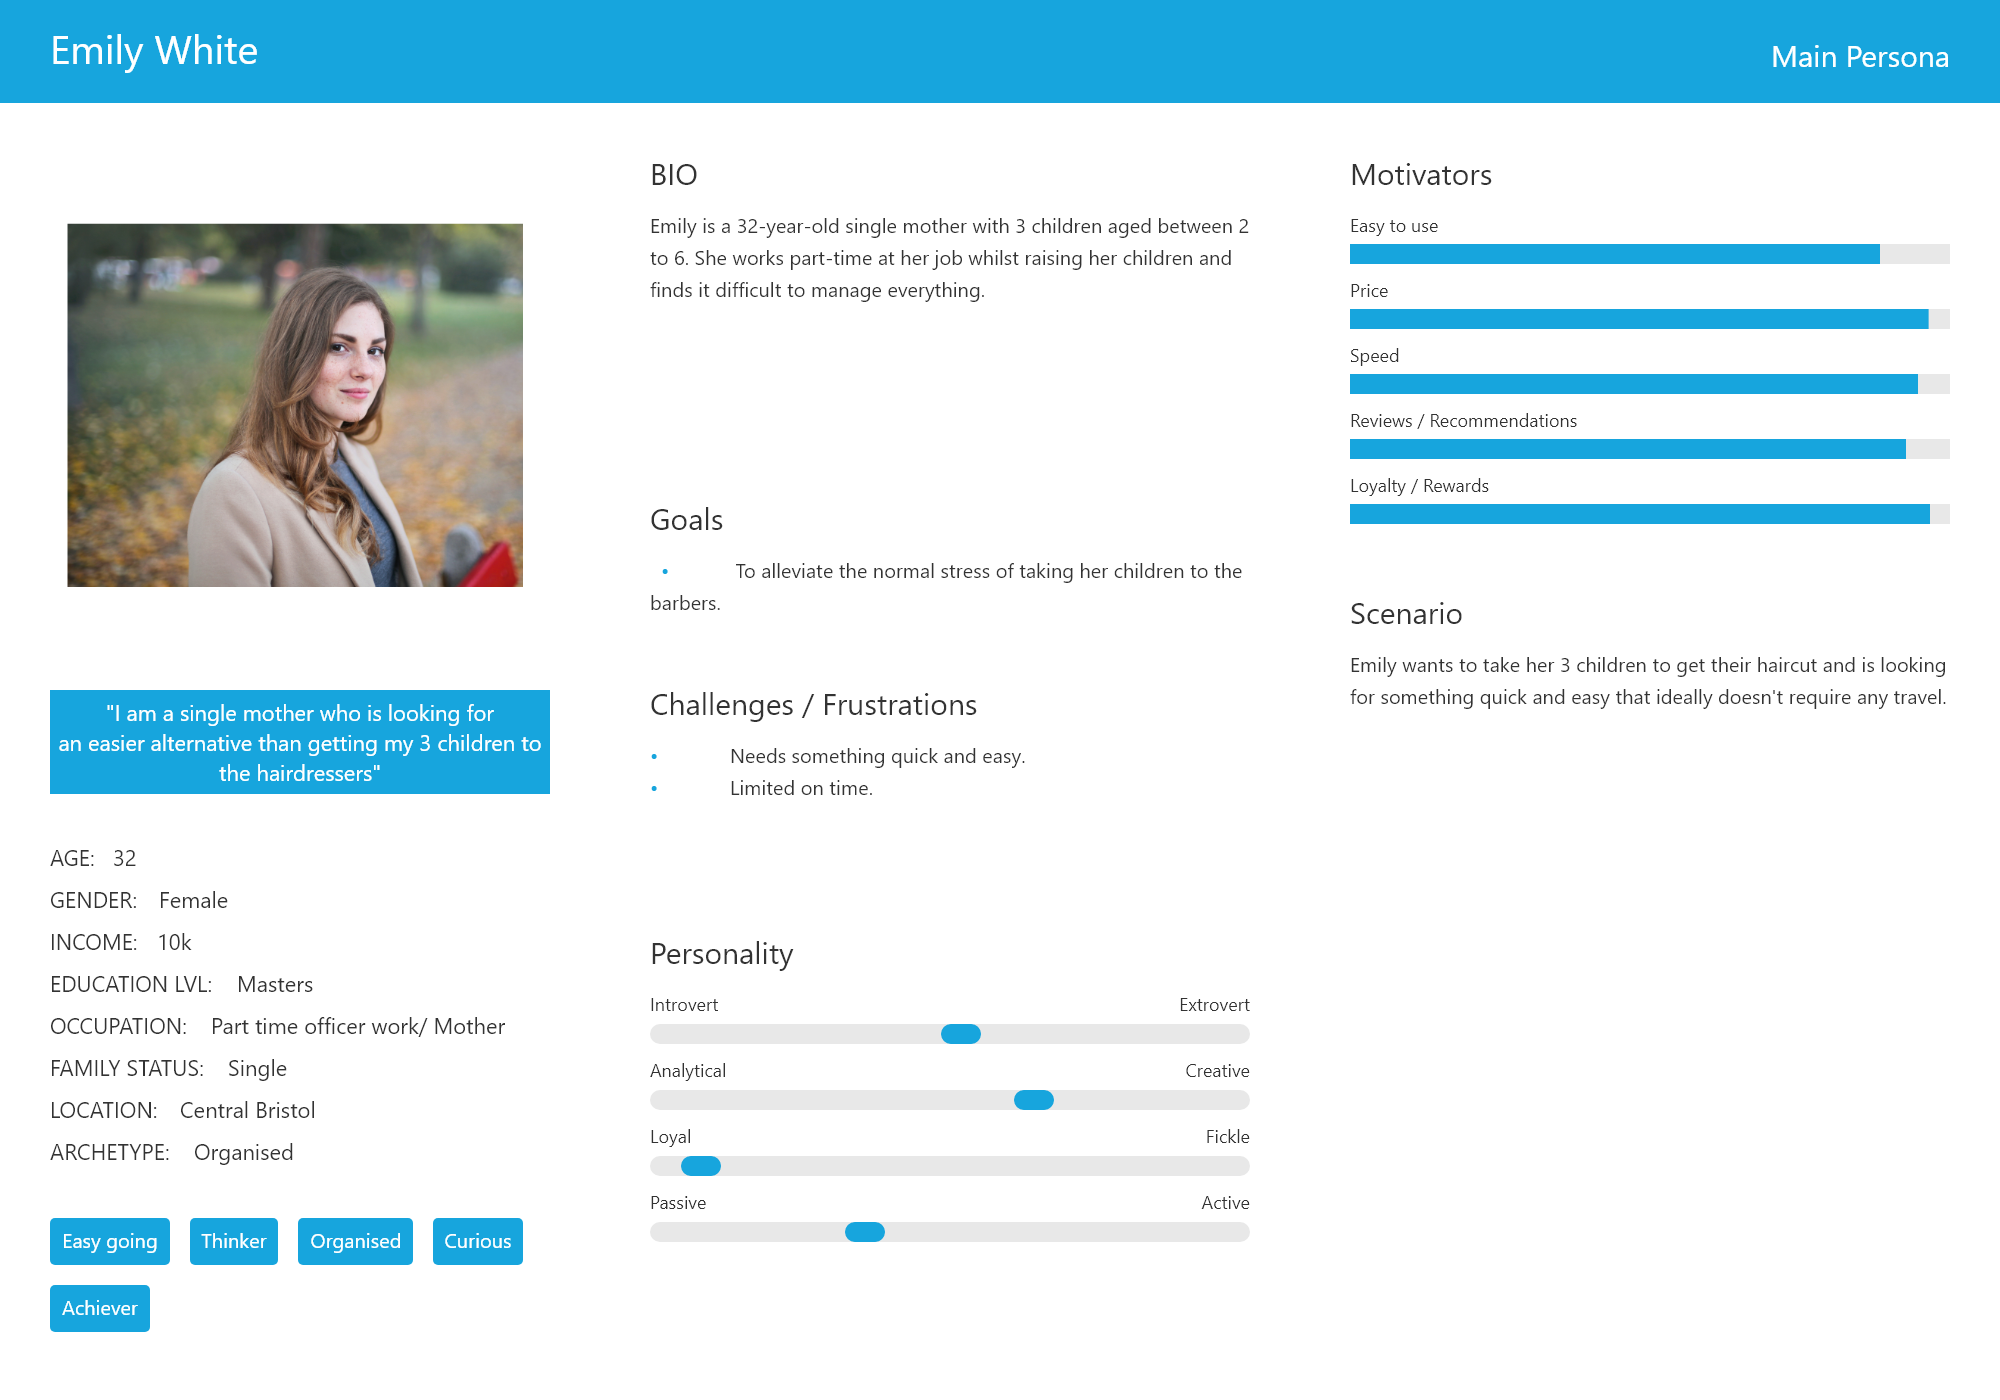
\includegraphics[scale=0.2]{images/persona_3.png}
			\caption{Persona 3}
			\label{fig:persona_3}
		\end{figure}
		
		\underline{Persona 4 - Alastair Craig}
		
		
		Profile: 
		\begin{figure}[H]			
			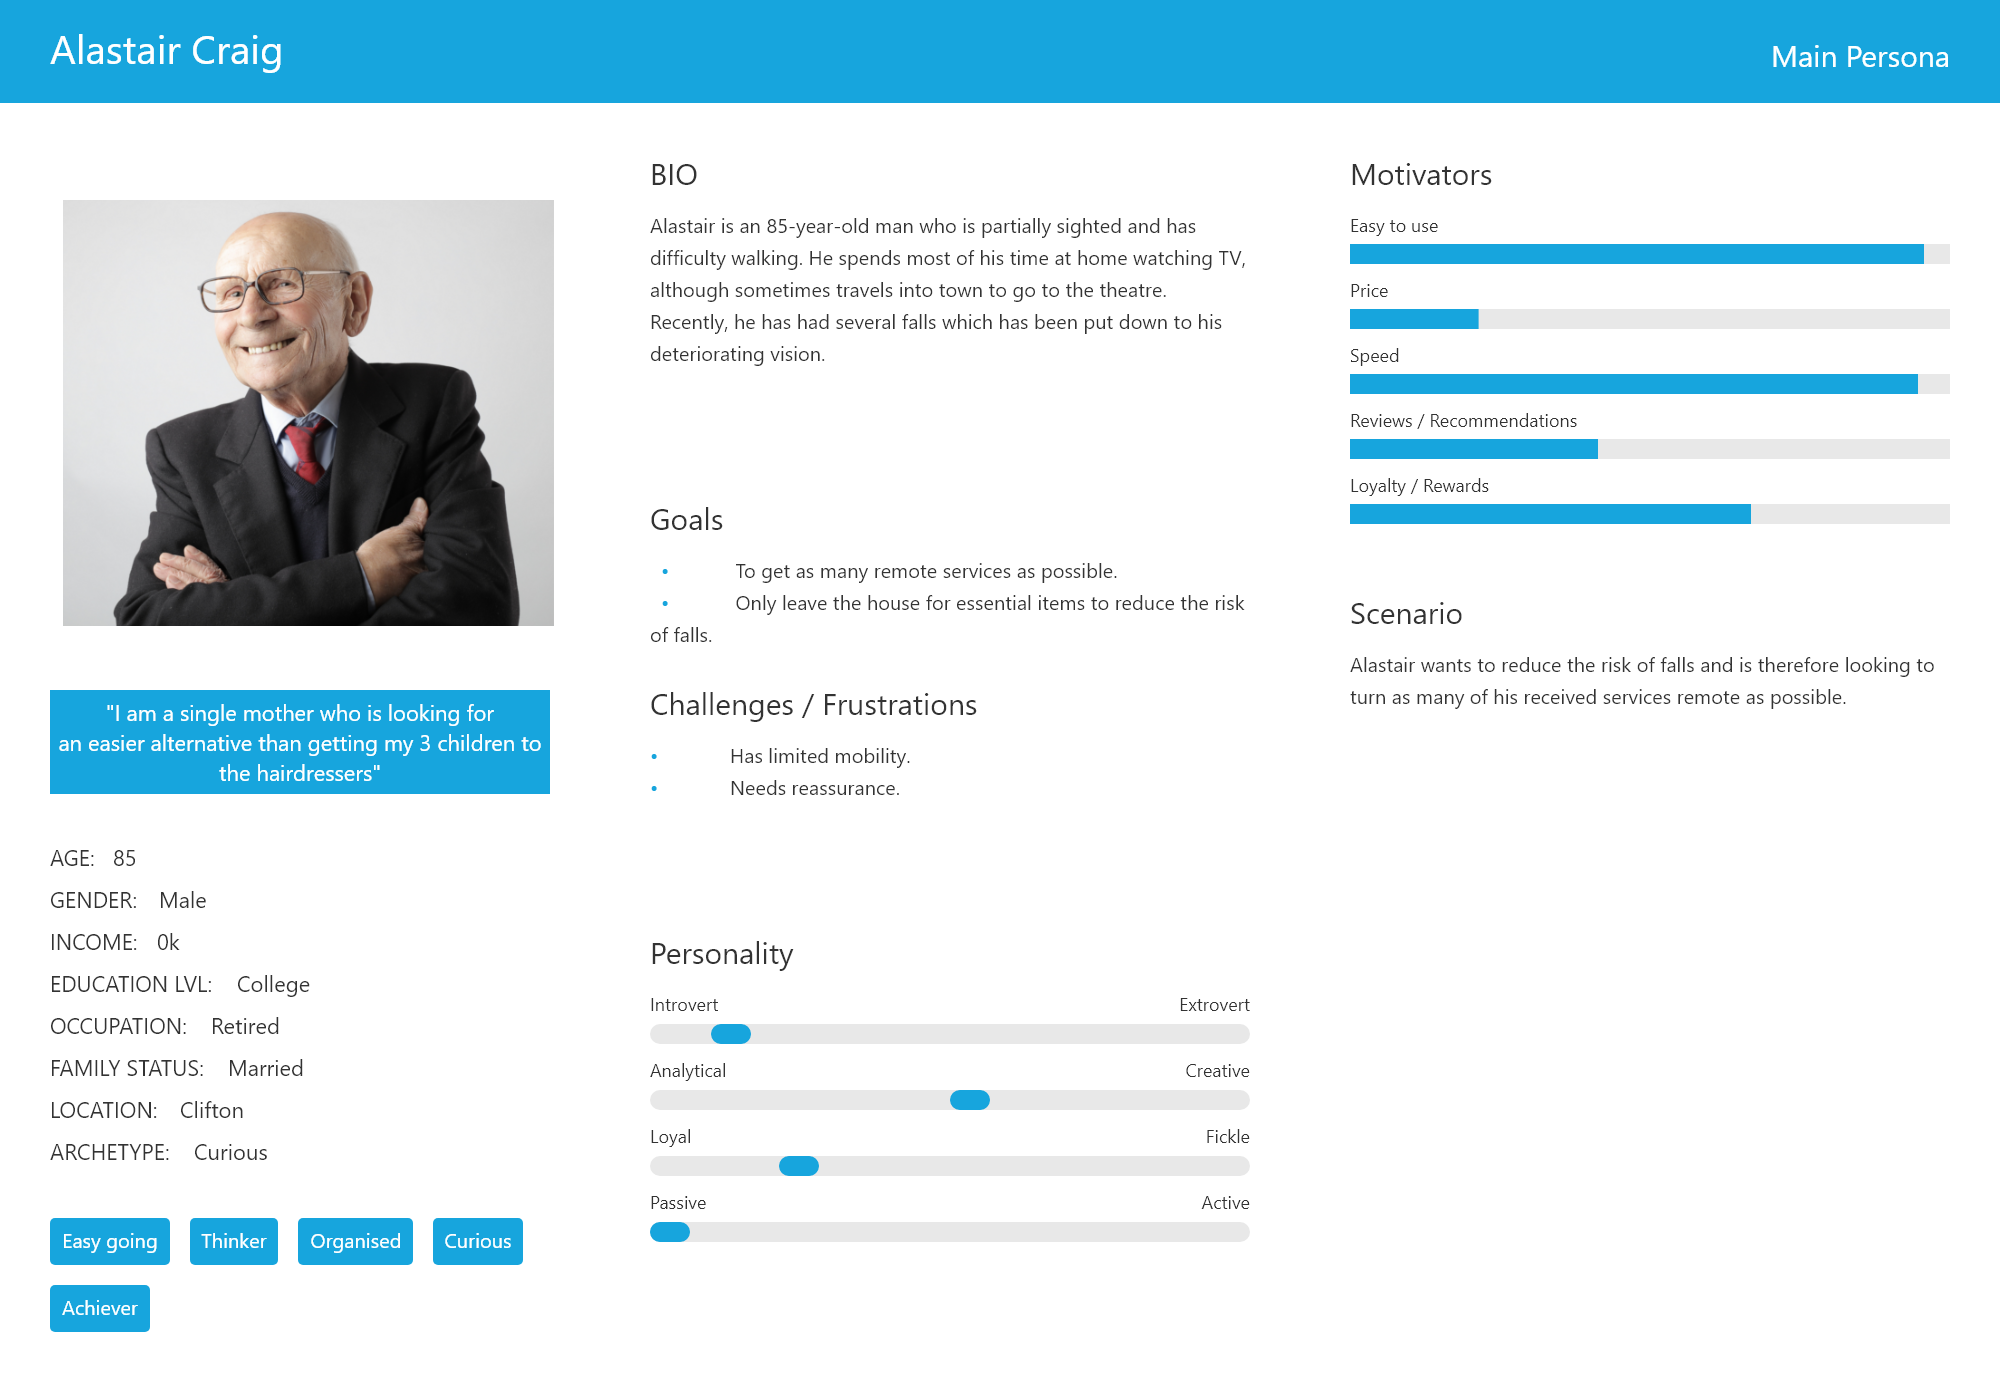
\includegraphics[scale=0.2]{images/persona_4.png}
			\caption{Persona 4}
			\label{fig:persona_4}
		\end{figure}
			

	\section{Software Requirements}
	Here we discuss and outline the software requirements, for which this section is similar to that found within a software requirements specification (SRS) document and lays the framework for the entire project. Here we discuss the application scope, user needs, functional and non-functional requirements, along with use cases.
	

	\subsection{Application Scope}
	The scope of the project was to create a fully working and functional barber application with several features, which are discussed in the User Needs below. To further aid in scoping the project, epics were created, which were further split into stories that could be carried out. Although it could be argued that this type of agile methodology is more relevant when working within a team of developers, it helped to determine a stringent workflow and timeline and aided in project delivery.
	The scope was then further defined when wire-framing in Adobe XD, which allowed for the first tangible design to be made.
	
	\subsection{User Needs}
	$\bullet$ Allow the application to run on a mobile device.
	\\
	$\bullet$ Allow the user to book a beauty treatment to receive at their home address.
	\\
	$\bullet$ Allow a barber to set up an account and specify their product details.

	\subsection{Requirements}
	\subsubsection{Functional Requirements}
	
	\begin{itemize}
		\item Customer-side Application
		\begin{itemize}
			\item The application shall allow a customer to create an account and login
			\item The application shall provide the user with basic account management capabilities
			\item The application shall allow for the user to pick from a range of relevant products and add them to their cart
			\item The application shall allow the user full management of their shopping cart
			\item The application shall provide only geographically relevant barbers and products to the user
			\item The application shall allow the user to view their past orders
			
		\end{itemize}
	\end{itemize}

	\begin{itemize}
		\item Barber-side Application
		\begin{itemize}
			\item The application shall allow a parent barber to create an account and login
			\item The application shall allow for integrated back-end management of it's barbers and products
			\item The application shall allow for the parent barber to view its orders
		\end{itemize}
	\end{itemize}
	
	\subsubsection{Non-Functional Requirements}
	
	\begin{itemize}
		\item Performance
		\begin{itemize}
			\item The application shall take no longer than 3 seconds to load the users home screen
		\end{itemize}
	\end{itemize}

	\begin{itemize}
	\item Data
	\begin{itemize}
		\item The application shall cache data where possible
		\item The application shall minimise calls to the database and make them only when relevant
	\end{itemize}
	\end{itemize}

	\begin{itemize}
		\item Use-ability
		\begin{itemize}
			\item The application shall follow nielsen's usability heuristics and be easily usable for the user without any guidance or help
		\end{itemize}
	\end{itemize}

	\begin{itemize}
		\item Security
		\begin{itemize}
			\item The application shall ensure that all app data be secured and encrypted
			\item The application should use OAuth for access delegation
		\end{itemize}
	\end{itemize}

	\begin{itemize}
		\item Operating System
		\begin{itemize}
			\item The application shall run on both iOS and android devices
			\item The application shall run on all devices newer than android 5.0 (API 21) - around 94.1\% of android devices
			\item The application shall run on all devices newer than iOS 9.0 - around 99.6\% of iOS devices
		\end{itemize}
	\end{itemize}

	
	\subsection{Use Cases}
	Here the use cases are presented, which are described by Ivar Jacobson as “a description of a set of sequences of actions and variants that a system performs that yield an observable result of value to an actor.” (Jacobson, et. al., 1999, p.41). Use cases are useful in the sense that they provide a structure for collecting customer requirements and setting the scope \cite{larsonUseCasesWhat2004}. They also allow for validation of the project through post-production testing, which can be seen in section \autoref{use-case-implementation}.
	\\
	
	To produce the use cases we reference both the user personas created in \autoref{user-personas} and the functional and non-functional requirements discussed in the previous section. Below lists the most pertinent use cases.

	\begin{itemize}
		\item Use Case 1 - \textcolor{blue}{\hyperref[chap:use-cases-1]{Sign Up}}
		\item Use Case 2 - \textcolor{blue}{\hyperref[chap:use-cases-2]{Login}}
		\item Use Case 3 - \textcolor{blue}{\hyperref[chap:use-cases-3]{Book a Haircut}}
		\item Use Case 4 - \textcolor{blue}{\hyperref[chap:use-cases-4]{Search for a Barber}}
		\item Use Case 5 - \textcolor{blue}{\hyperref[chap:use-cases-5]{Checkout}}
		\item Use Case 6 - \textcolor{blue}{\hyperref[chap:use-cases-6]{View Orders}}
		\item Use Case 7 - \textcolor{blue}{\hyperref[chap:use-cases-7]{Sign Out}}
		\item Use Case 8 - \textcolor{blue}{\hyperref[chap:use-cases-8]{Add a Barber}}
		\item Use Case 9 - \textcolor{blue}{\hyperref[chap:use-cases-9]{Add a Product}}
	\end{itemize}
	
	The above use cases are further designed in \autoref{chap:use-cases}.

	
	\section{System Design}
	In this section, we discuss the structure of the project, the system and software architectures and data and state management given the previously specified requirements. 
	
	\subsection{Domain Model}
	TODO: discuss domain model
	Domain driven design (DDD), which originated from a 2003 book by Eric Evans \cite{evansDomainDrivenDesignTackling2003} depicts a paradigm whereby data is visualised as a lexicon of abstractions, with the data model clearly representing key data concepts and the relationships between them. Modelling in this way bridges the gap between activities and interests of the users with the software and allows.
	
	
	\begin{figure}[H]
		\centering
		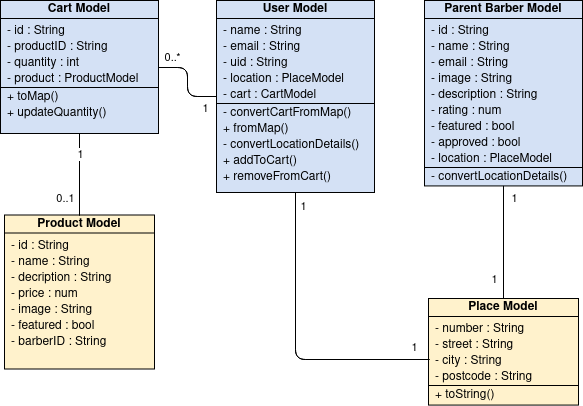
\includegraphics[scale=0.7]{images/model-class-diagrams.png}
		\caption{Model Class Diagrams}
		\label{fig:model-class-diagrams}
	\end{figure}
	
	\subsubsection{Entities}
	
	Within DDD it is recommended that a structured architecture is implemented, which is discussed in detail below.
	
	TODO: continue with article	and discuss how the project code was split using DDD, i.e. models, screens etc etc
	
	\subsection{System Architecture}
	https://www.raywenderlich.com/6373413-state-management-with-provider
	System Architecture can be broadly defined as a conceptual model which outlines the structure, behaviour and interactions between internal and external components of the system. Modelling and creating a structured and well-defined architecture allows for the development of a sustainable, scalable and stable software product which can easily grow relevant to the demands placed on it's features.
	
	The overall system architecture can be seen below in figure \ref{fig:system-architecture}.
	
	\begin{figure}[H]
		\centering
		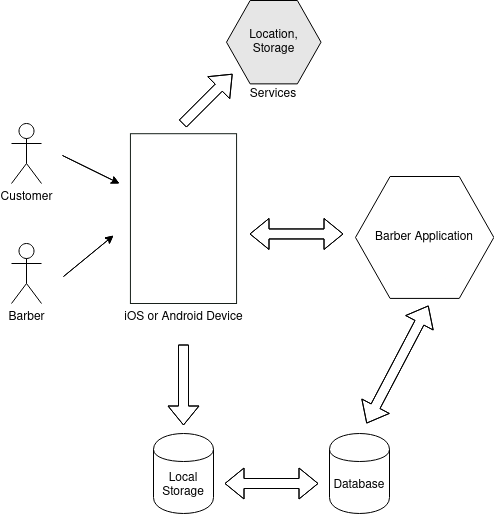
\includegraphics[scale=0.7]{images/system-architecture.png}
		\caption{High-level System Architecture}
		\label{fig:system-architecture}
	\end{figure}
	
	When designing the architecture, core business logic was kept separate from the UI, database and network. For example, when interacting with the database the UI called upon the utilities package and any API calls where contained within the providers package. The project was also split into 3 layers, according to clean architecture principles (\cite{martinRapidApplicationDevelopment1991})
	
	\begin{itemize}
		\item Presentation layer
		\begin{itemize}
			\item Screens - Contains unique UI elements
			\item Widgets - Elements that are used to create the UI and feed into the screens
		\end{itemize}
	\end{itemize}
	
	\begin{itemize}
		\item Domain layer
		\begin{itemize}
			\item Utilities - Contains business logic and elements that are used to make calls to the database or interact with any external APIs.
			\item Providers - State management tools that are called on throughout the application.
		\end{itemize}
	\end{itemize}
	
	\begin{itemize}
		\item Data layer
		\begin{itemize}
			\item Models - Contains the models used for local storage.
		\end{itemize}
	\end{itemize}

	 This generally follows clean architecture principles (\cite{martinRapidApplicationDevelopment1991}) and each layer is represented in figure \ref{fig:clean-architecture} below.
	 
	 \begin{figure}[H]
	 	\centering
	 	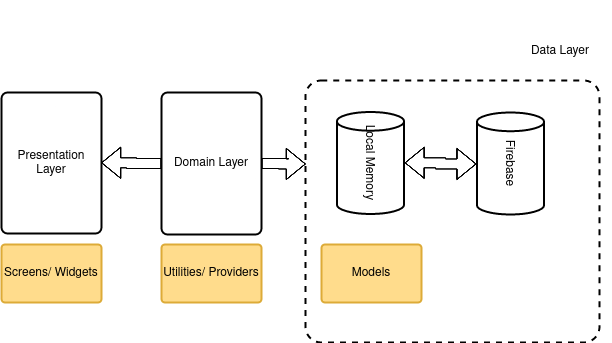
\includegraphics[scale=0.7]{images/clean-architecture.png}
	 	\caption{Clean Architecture (adapted from \cite{martinRapidApplicationDevelopment1991})}
	 	\label{fig:clean-architecture}
	 \end{figure}
 
 	From this architecture and the previously devised specifications, an activity diagram was created, to detail the minimum required activities within the application, which can be seen in figure \ref{fig:activities} below.
 	
 	
 	\begin{figure}[H]
 		\centering
 		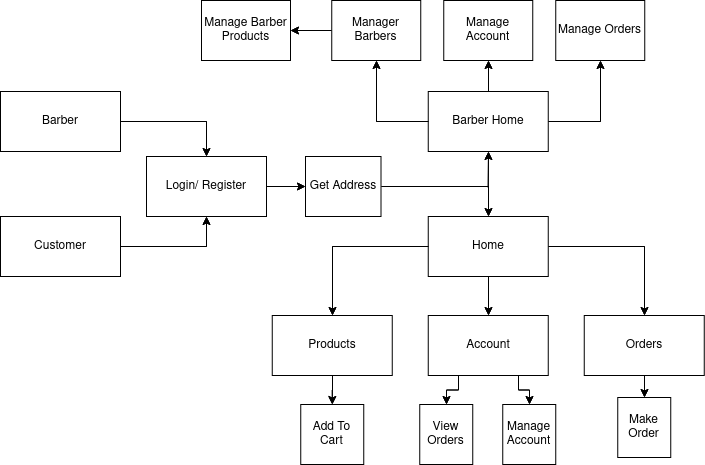
\includegraphics[scale=0.6]{images/activities.png}
 		\caption{Application Minimal Activity Diagram}
 		\label{fig:activities}
 	\end{figure}
	 
	

	
	\subsection{Client-side Specification}


	
	\subsubsection{State Management}
	State management is an important feature within flutter. As flutter is declarative, rather than allow for changes in the widget or UI, each time a change is required the UI is rebuilt to reflect the applications current state. Within flutter there exists a variety of different methods for managing the state of the app, of which Provider, BLoC and GetX are some of the most popular and widely used. Here we will discuss the merits and pitfalls of each before settling on a framework for the application for both the local and global scope.
	\\
	
	\noindent \underline{Provider}
	\\
	\noindent
	By far the most commonly used state management framework is Provider, a wrapper for the InheritedWidget class, which works by exposing all of the relevant daughter widgets to a value, so that data can be created, listened to and disposed of globally. To do this, a class is first created that extends 'ChangeNotifier', which allows classes 'subscribe' to the senders data. Then, through using the method 'notifyListeners()' all of the daughter widgets will be updated with the current value and the UI rebuilt.
	
	One negative of Provider is that it is only optimised for relatively few listeners, with it being $\mathcal{O}(n^2)$. With large applications and where speed is important this could be an issue.
	\\
	
	\noindent \underline{BLoC}
	\\
	BLoC is a state management tool within flutter that is based on event driven states. For example, when adding to the basket you could trigger and AddBasketState, before checking out and triggering a CheckoutState. The benefit of this is that the code becomes fairly inflexible, which in a team working environment could reduce the risk of accidental bug implementation.
	
	BLoC is also beneficial in acting to separate the logic from the widgets, which aligns with the previously discussed architecture principles.
	\\
	

	\noindent \underline{GetX}
	\\
	\noindent
	A large benefit of GetX is that, unlike Provider and BLoC, it acts not only as a state management tool, but as a "micro framework". For example, one does not need to access the widget tree and context to navigate between routes, allowing for seamless navigation between pages and also finding the object anywhere using 'Get.find(), allowing for more separation between the business and presentation logic. Not needing to access context means that GetX also allows for dependency injection separate from using inheritedwidget, which removes unnecessary boiler plate code and aids in speed.

	
	\subsubsection{Provider}
	For locally managing state, 'setState()' can be utilised within a statefulWidget, which was used extensively throughout the project, for example in the Checkout screen when updating the total to match the given products.
	
	For managing the global state within the project it was decided that Provider would be used as the primary global state management framework for several reasons. Firstly, it is fairly simple to understand, and when used with ChangeNotifier allows for the required state management for the proposed application. Secondly, Provider lends itself to a clean architecture with the logic seperated from the UI, meaning that a simple widget tree can be designed and implemented, which can be seen in figure \ref{fig:widget-tree} bellow, which displays the widget tree diagram for the application. Unlike BLoC, Provider allows for good flexibility, which as there was only 1 developer on the project makes more sense, giving greater scope for changes throughout the project. Despite this, future growth could lend itself towards also implementing BLoC alongside Provider, to improve structure and increase growth potential, a good example can be seen with Ebay's Motor App \cite{techblogEBayMotorsState2021}.
	
	 Finally, although GetX makes an excellent framework for larger projects, due to it's "micro framework" that encompasses several features not limited to controlling state management, the fairly simplistic nature of Provider better suited the relatively small project and hence was chosen here. The overall state management can be seen in the implementation section in \ref{fig:widget-tree}.
	 	
	 	
	


	\subsubsection{Deciding on a Framework}
	There exists a variety of software architectural frameworks, although not exhaustive this includes Client-server, Peer-to-peer, Microservices and Model-view controller (MVC). For this project, we decided to go with MVC as the architectural framework, which, for brevity is the only discussed here.
	Used the screens as the view
	Used ChangeNotifier as the controller
	TODO: talk about MVC
	
	\section{Prototyping}
	An essential component of UCD and more generally UX design is prototyping, which involves making mock-ups of the application that act as early prototypes to influence later development \cite{arnowitzChapter15Wireframe2007}. Mobile app prototyping has many benefits to the project, including:
	\begin{itemize}
		\item Validates strategic design directions of the product
		\item Saves time by discovering any constraints early in the project
		\item Allows for early, interactive user testing
		\item Acts as a template for the UI during the implementation phase
	\end{itemize}
	 
	
	The prototyping for the application involved two distinct stages; firstly, an initial sketch was done with pen and paper to discern the layout and overall themes associated with the app, before a wireframe was created to further define the prototype and allow for early testing.
	
	\subsection{Initial Sketches and Brainstorming}
	Initial sketches involve using pen and paper to elucidate problems and brain storm ideas for the project. During this phase, several design and UI features were considered, which allowed us to generate many ideas, using a fast and simple approach.
	
	Some of these sketches can be seen in figure \ref{fig:sketches} below.
	\begin{figure}[H]
		\centering
		
\includegraphics[scale=0.3]{images/placeholder.jpg}
		\caption{Pen and Paper Sketches and Brainstorming}
		\label{fig:sketches}
	\end{figure}
	(TODO: UPDATE PHOTO WITH INITIAL SKETCHES)
	
	\subsection{Wire-framing}
	Once the sketches were completed we moved on to wire-framing the application, which involved taking the best sketch variants and creating a more detailed, lower level prototype.For the wire-framing application Adobe XD was chosen for several reasons. Firstly, it has strong prototyping functionality, allowing the user to click around the application through the use of ‘components’. This interactivity means that early testers can get a real feel for how the application works. An illustration of this can be seen below, whereby each arrow represents a state change in the form of a trigger/ action pair, whereby for example a user could click on ‘Available Right Now’ and be taken to the ‘Checkout’ as seen in figure \ref{fig:prot-comp} below.
	\begin{figure}[H]
		\centering
		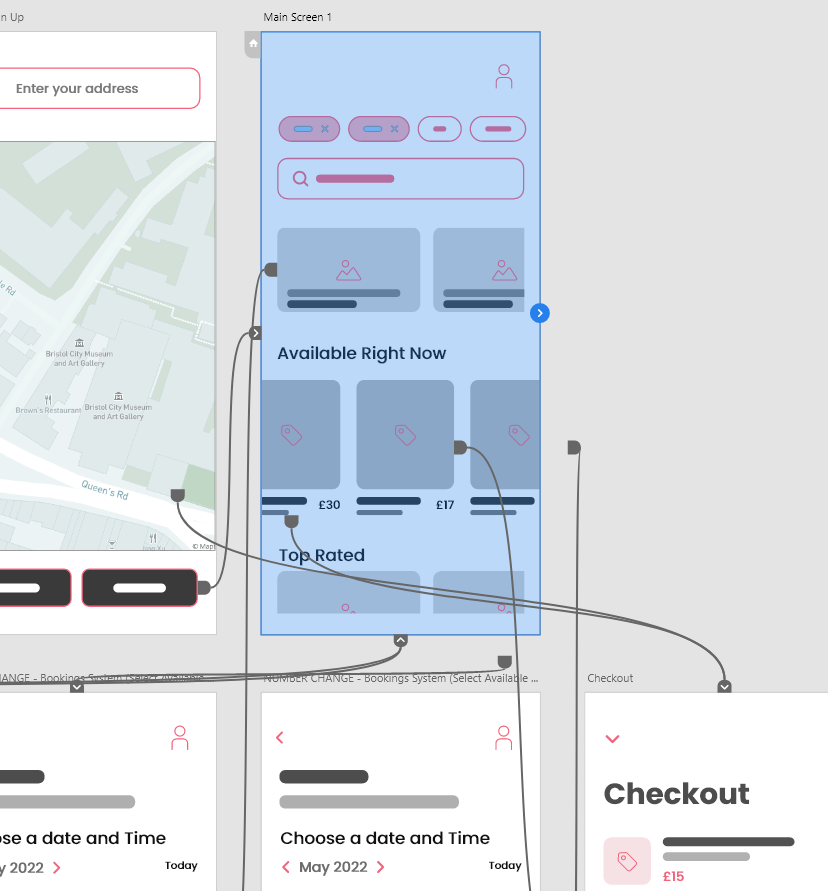
\includegraphics[scale=0.5]{images/prototyping-components.png}
		\caption{Component Interactivity within Adobe XD}
		\label{fig:prot-comp}
	\end{figure}
	
	
	Adobe XD also allows for easy distribution of the prototype in the form of a shareable link that opens in the browser and encompasses the same functionality and components that can be found within the application itself, meaning that anyone with access to a browser can test the prototype. Along with this, the prototype also allows for comments to be made, which are fed back to the owner. This comment capability was used early on during beta testing when it was sent out with the early questionnaire and influenced initial design decisions \cite{SketchVsFigma0200}.
	
	When designing the screens there was a strong focus on user experience following Nielsons 10 Heuristics for User Interface Design \cite{experience10UsabilityHeuristics} . For example, the functionality was kept as minimal as possible to avoid clittering and avoid cognitive load on the user, the user was given control to go back and forward between previous screens to allow for user control and freedom and simple and self-explanatory language was used to apply recognition over recall. For example, the Sign In screen below extraneous text was kept to a minimum by using images for the login items, such as Google, Facebook and Twitter, a sign up button was included to allow the user to access the application through creating a new account and large, clear sign in forms and buttons were used. The full interactive Adobe XD wireframe can be found \href{https://xd.adobe.com/view/c6aeda9c-9b9a-456a-b699-cc4cd8b4cefa-93fd/}{here}. 
	
	\begin{figure}[H]
		\centering
		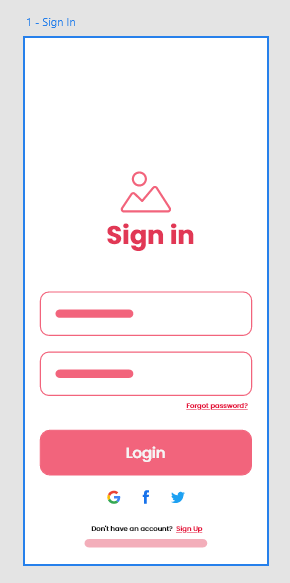
\includegraphics[scale=0.85]{images/sign-in.png}
		\caption{Sign In Page Made With Adobe XD}
		\label{fig:sign-in}
	\end{figure}
	
	\section{Implementation}
	Here we discuss the implementation of the application, which is divided into separate sprints, each of which pertains to a relevant feature within the application. Finally, we address the implementation each use case individually.
	
	\label{chap:implementation}
	\subsection{Setup}
	Before beginning the development sprints, the first task involved setting up the developer environment. To code the application it was decided that an integrated development environment (IDE) was used due to the comprehensive features it provides to aid in development and maximise productivity. For this, it was decided that the IDE 'Android Studio' by JetBrains \cite{DownloadAndroidStudio} was to be used, due to previous experience and familiarity with other JetBrains applications, along with Android Studios excellent built in features and seamless integration with flutter. 


	\subsubsection{File Structure}
	Although there is no official recommendation for structuring the app, here we follow a commonly used scheme which aligns with the previously discussed architecture principle and includes models; the files that serve as collections of data that are used in conjunction with the widgets to form the user interface of the application; providers, which inhabit the state management tools of the application; screens, which display the UI of the app; utilities, which are used to connect to the back-end; and widgets, which contain the business logic of the app.
	
	
	
	\subsection{Sprint X - UI}
	The first sprint involved implementing the UI, which was previously wire-framed within Adove XD. Flutter offer an Adobe XD plugin to turn wireframes directly into code, however, this was not used for several reasons. In Adobe XD components are positioned absolutely, whereas in Flutter it is done relatively, leading to several issues with positioning that would not scale. Adobe XD also does not contain customer properties and therefore mapping these to components, such as title is not possible, therefore the UI was implemented manually.
	
	Within Flutter, the UI is built through using widgets, which describe not only the look of the application, but also provide the state and can be rebuilt to reflect a change in state. As an example we can look at the forgot password screen, a segment of which is shown in \ref{code:forgot-password}. The UI here is built using a variety of widgets. For example, line 2 shows a Column widget, which allows for daughter widgets to be stacked alongside each-other vertically. The first daughter widget is a TextField that allows us to get text from the user and this is wrapped within a padding widget, which allows us to specify the required padding to aid in UI design. Finally, a button is placed within the application using the GestureDetector widget, which, by implementing the 'onTap' function looks for input from the user and then navigates to the Login screen after using the AuthenticateProvider to send a password reset link.  
	
	
	\subsubsection{Cupertino vs Material}
	A consideration when building the UI was on whether to model the application using Cupertino, which gives the app an iOS type look and feel or material, which is more generalised across android and iOS. As the project was designed to be multi-platform, it was decided that material would be used throughout. 
	
	Using material also lends itself well to the project for other reasons, For example, it gives us access to a number of useful widgets at the root of the application. For example, the Navigator allows us to keep a track of the users chosen screens as a stack and by using Navigator.pop() and Navigator.push() we can navigate between screens. This is implemented in the Navigate widget, which can be seen in appendix \ref{code:navigate} and allows us to easily navigate the user around the application. Using material also gives us access to both a bottom navigation bar, which can be seen in appendix \ref{code:nav-bar} and a side bar. Finally using material allows for easy styling of the app by using the built in class 'ThemeData'. The implementation of material can be seen in the main.dart file in appendix \ref{code:MyApp} which serves as the root and entry point to the application.
	
	
	
	\subsection{Sprint X - Sign Up and Login}
	Once the UI was built the Login and Sign Up page logic was implemented. This involved creating an authentication page (aunthenticate.dart), which acted as a provider for the user and other authentication logic that could be injected into the UI along with using a database to store users so that user data could be persistent.
	
	\subsubsection{Authentication}
	\label{authentication}
	Firebase has its own built in authentication library \cite{FirebaseAuthentication2021}, which works by providing email and password based authentication along with OAuth 2.0 capabilities, both which were used extensively throughout. Firebase Authentication was used for the project due to several considerations -
	\begin{itemize}
		\item Excellent built in security features
		\begin{itemize}
			\item Can easily restrict access to different specified groups within an organisation
			\item Security is enforced by server-side rules, limiting unsafe usage within the app itself
			\item Uses token generation to ensure confirmed data
		\end{itemize}
		\item Integration with firebase database and storage
		\item Easy modification through Googles declarative language
		\item Excellent integration with OAuth 2.0
		\begin{itemize}
			\item Using OAuth allowed for sign in methods with Google, Facebook and Twitter to align with the previously drawn wireframes
		\end{itemize}
	\end{itemize}
	
	
	\subsubsection{Sign Up}
	The user is first presented with the sign up screen whereby they can enter their name, email and password and click through to make an account. Once the user clicks the Sign Up button, a token is created within Firebase Authentication and the credentials are stored. Inside of authenticate.dart there is a signUp method which carries out the logic behind user sign up, which works in several steps.
	\begin{itemize}
		\item First, a UserCredential (which holds the return value of firebases sign up method) is returned from an attempt to create a new user with the email and password
		\item Next, a created model (UserModel, which can be seen in appendix \ref{code:user-model}) is assigned to the user which holds all pertinent information, such as name, email, shopping cart items etc
		\item The Authenticate enum status is set to AUTHENTICATED as discussed below
	\end{itemize}
	

	
	\subsubsection{Login}
	Once the user has been created and the credentials are stored, the user can login using the given name and password. This is then authenticated with Firebase and a response is returned to the client, before the user is then logged in for the session. To follow the authentication status of the application we created an enum seen in figure \ref{fig:authenticate-enum} below. This can then be tracked by using 'Provider.of<AuthenticateProvider>(context)', allowing us to manage and alter the state of the application based on the status of the user.
	
	\begin{figure}[H]
	\centering
	\label{fig:authenticate-enum}
	\begin{minted}{dart}
		enum AuthStatus {
			UNINITIALISED,
			UNAUTHORISED_USER,
			UNAUTHORISED_BARBER,
			NOT_AUTHENTICATED,
			AUTHENTICATING,
			AUTHENTICATED,
			BARBER_AUTHENTICATED,
			AUTH_WITH_MAPS
		}
	\end{minted}
	\caption{Enum Found in authenticate.dart}
	\end{figure}
	
	The user can also be authenticated and signed in using Google sign in; for which the 'google\_sign\_in' package was utilised, Twitter sign in; for which the package flutter\_twitter\_login was used and Facebook sign in; whereby the package flutter\_facebook\_auth was used. All of these work by returning a respective OAuth token and therefore is a secure way to authenticate the user.
	
	
	Similar to when signing up, on login, a User Model is created, which locally stores the details needed for the user, i.e. id, name, email, address and any other relevant data such as their cart items within the Authenticate class. In this way, the data contained within can be accessed using Provider and data such as cart items accessed globally. Part of the user model can be seen in appendix \ref{code:user-model}.
	
	
	\subsubsection{State Management}
	
	TODO: move below figure in relevant place
	
		
	\begin{figure}[H]
		\centering
		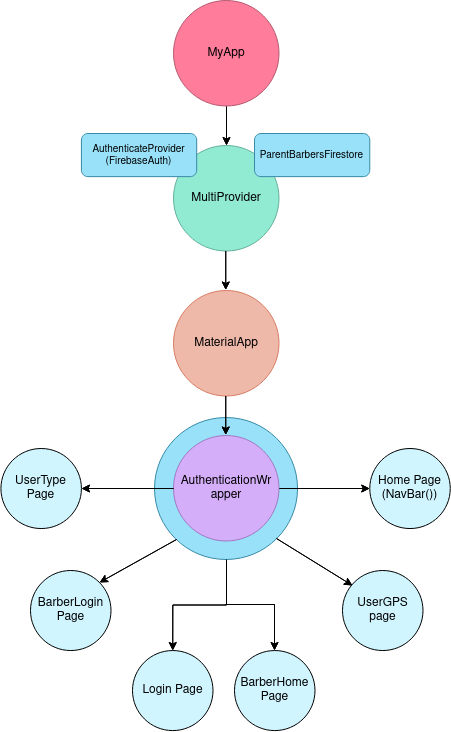
\includegraphics[scale=0.55]{images/widget-tree.png}
		\caption{Widget Tree Diagram}
		\label{fig:widget-tree}
	\end{figure}
	
	


	
	
	\subsection{Sprint X - Backend Design}
	The next sprint involved modelling and creating the database to suit the needs of the project. As previously discussed, for the project it was decided that a noSQL database, instead of a relational one was to be implemented.
	
	\subsubsection{Database Design}
	Although noSQL is most frequently used for non-relational data a database schema was constructed to constitute the parent barbers, barbers and products as modelling this way added to readability with the added benefit of the features previously discussed. The schema is represented in figure \ref{fig :database-schema} below.
	( TODO: add orders to the database schema)
	
	\begin{figure}[H]
		\centering
		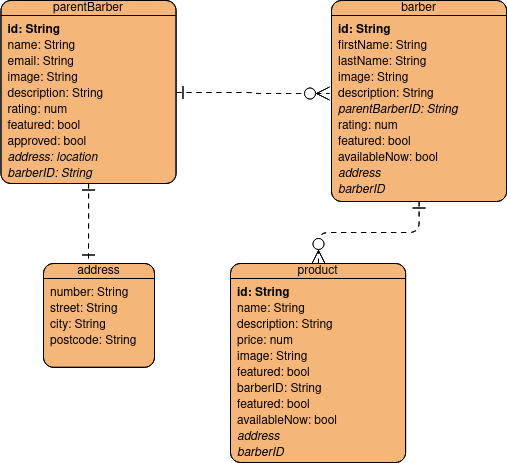
\includegraphics[scale=0.7]{images/database-schema.png}
		\caption{Database Schema}
		\label{fig:database-schema}
	\end{figure}
	
	Loading all parentBarbers/ barbers and products - 
	When entering the app it is more effecient to make one call to the server rather than multiple due to GPS restrictions. Therefore ParentBarbers, barbers and all of their products are loaded within a certain radius, rather than loading parentBarbers and barbers separately throughout the app. 
	
	Don't nest as calls will fetch all of the parent and nested structured so better to have separate data.
	
	
	Within the UserDatabase class, for the createNewUser function, we pass through the authentication uid, which is then used as the document id, so that future calls can refer to this and therefore fetch the document, without doing a call such as 
	\begin{lstlisting}
		_firebaseFirestore.collection(collection).where('uid', .isEqualTo('givenID')).get()
	\end{lstlisting}
	which does not scale well due to a search time of $\mathcal{O}$(n). Instead, we store the uid as the document id, allowing us to do a similar, although quicker call such as
	\begin{lstlisting}
		_firebaseFirestore.collection(collection).doc(userId).get()
	\end{lstlisting}
	which gives a search time of $\mathcal{O}$(1).
	
	
	
	\subsection{Sprint X - Connecting the Frontend and Backend}
	
	\subsubsection{Persistent Storage of the User}
	Although the above methods allow the user to login and sign up  along with locally store the data, there is no mentioned way to persistently store any user data.
	
	 
	
	
	To get the list of items within a range
	1) Get the users current location
	2) Query firestore with the radius
	
	\subsubsection{Loading the barbers}
	When loading the barbers either they were loading through making a database query based on the parentBarberId once the parent barbers were loaded, or every barber was loaded into memory and this was the filtered in memory.
	\\
	Pros of first method - Scales well as does not matter how many barbers there are
	\\
	Cons of first method - more costly as there are more requests to the db
	\\
	Pros of 2nd - cheaper
	\\
	cons - does not scale well
	
	\subsubsection{Shopping Cart}
	Chose to store the cart items in a nested array as this adds to readbility and structure and although this restricts look up time, this is not relevant due to the limited number of items a user will order.
	
	\subsubsection{Checkout}
	Similar to section \ref{authentication} to create a search time of $\mathcal{O}$(1) a seperate 'orders' collection was created, with each document representing all of the pertinent order details. Within each barber and user, the document (order) id was then added to each respective order arrays, for quick and easy lookup.
	
	\subsection{Sprint X - Location}
	https://firebase.google.com/docs/firestore/solutions/geoqueries
	Once the user logs in they give their location in the form of their address. This is stored in 'geohashes', which are longitude and latitiude co-ordinates that are hashed into a single Base32 string. Each character presents a greater level of precision and therefore we opted for 9, which represents an area of 5 x 5 meters.
	
	User location access is granted through the following line in the ./android/app/src/main/AndroidManifest.xml file
	\begin{lstlisting}
		<uses-permission android:name="android.permission.ACCESS_FINE_LOCATION"/>
	\end{lstlisting}
	For the search results we use a drop down menu in the form of flutters built in 'showSearch' function loosely following a guide on medium \cite{sheanLocationSearchAutocomplete2020} to display a search page and 'SearchDelegate' to define the content of said search page.
	
	A textEditingController is used to collect the inputted data from the user and pass through to the showSearch function.
	
	\noindent
	
	
	
	\subsubsection{Autocomplete locations}
	As a means for the user to autocomplete their address when signing up, the 'Place Autocomplete service' within the Google Places API, which returns location predictions in response to HTTP requests was implemented using a request adhering to a set of parameters, the full list, along with details of the API can be found on the Google Developers website \cite{PlaceAutocompleteRequests}.
	First, we enable the Places API within the Google console, before we then create a location model which can hold the data returned from the API. We then create an API request using the above aforementioned API format. For brevity, not every option is discussed, but those of importance include 'input', which is the user query, 'types', which determines the query returned, for which we specify address as we wish to fetch the users full address and a session token, which is required for each new query. The query can be seen here:
	\begin{lstlisting}
		'https://maps.googleapis.com/maps/api/place/autocomplete/json?input=$input&types=address&components=country:uk&lang=en&key=$apiKey&sessiontoken=$sessionToken'
	\end{lstlisting}
	The returned results are in json format and after some minor error checking we parse using json.decode into a list with our LocationModel class, whilst assigning a new UUID for each query (Google recommends to use version 4 UUID and so this is used here). Without our 'user\_gps.dart' file
	
	For the content of the search page we use pass in newly created session token into the ShowSearchPage class, which in turn sends an API request and parses the json data to return a list of locations in the form of 'place id's' and 'description' using a FutureBuilder. From here, we pass through the location id to the getLocationDetails function to fetch the address details of each location and put into a PlaceModel object.
	
	Next, we parse the data into JSON format by passing the PlaceModel object into the function 'createLocationMap', which creates a map using the location data. Finally we pass through this map to the 'addLocationDetails', which uses the given user id to update the database with the users location.
	
	\subsection{Sprint X - Barber Side Application}
	The next sprint involved..
	In order to create a comprehensive application the final sprint involved coding a barber side app, giving the ability for the barber interact with the database and allow them to create an account, add and remove barbers and view orders.
	
	\subsubsection{Creating a Parent Barber}
	As the location functionality of the application requires both longitude and latitude co-ordinates, along with a geohash (EXPLAIN HOW PLUGIN USED TO GET THIS).
	
	\subsection{Widgets, Common Items and Added Features}
	Here we discuss any items not covered within a specified sprint.
	
	\subsubsection{Widgets}
	Several widgets were used to increase readability and brevity of code. For example, 'return\_text.dart' allows for access to the main components of the Text function and 'return\_image.dart' allows for easy use of the NetworkImage function, giving brevity and readability to the code.
	
	\subsubsection{Common Items}
	The common items contains global variables that were accessible throughout the project. Initially this included structures and arrays that served as objects to test the functionality of the frontend, for example a barber shop class with a nested list of barbers classes, each with a name, age, description etc. As backend functionality was added these items were removed. A theme class was then added which contains dart files that can be implemented. Doing it in this way meant that the application could be easily styled, without any unnecessary refactoring of code.
	
	\subsubsection{Launcher Icons}
	Created using GIMP. Plugin flutter\_launcher\_icons used to install icons across android and iOS
	
	\subsubsection{Discount Codes}
	
	\subsubsection{Hide and Show Password}
	
	
	
	\section{Testing}
	\label{use-case-implementation}
	\subsection{User Testing}
	\subsection{Acceptance Testing}
	\cite{humbleContinuousDeliveryReliable2010}
	It is recommended that acceptance testing is used throughout development as a metric to ensure a continious link between the customer and development and is an important tool within UCD. To implement this, here we analyse against the previously defined use cases as set out below.
	
	\subsection{Use Cases}
	TODO: refer to screenshots of app in use cases
	
	\section{Conclusion and Further Work}
	\subsection{Conclusion}
	The motivation for this project was to create a cross-platform working MVP of a delivery barber app that attained the required objectives as stated in the introductory chapter, which are addressed here.
	\newline
	
	\noindent
	\underline{Conduct Research to elucidate any market gaps}
	\newline
	
	\noindent
	I begin the thesis by discussing the methodologies that will be utilised throughout the project, for example new product development - which encompassed the stages involved to bring the app from ideation to market and agile, which was used as a more general project management tool to guide the work. In section \ref{market-analysis} I then go on to discuss existing applications in the field, any market gaps and define the novelty of the proposed application. I therefore believe that this first objective was met well.
	\newline
	
	\noindent
	\underline{Through a user centric design methodology plan and prototype the}
	\\
	\underline{user interface of the application} 
	\newline
	
	\noindent
	After discussing market gaps I then go on to decide on which platform best suits the application which can be seen in section \ref{chap:platform}, where I also discuss the most suitable software modalities, including frontend and backend platforms. I then move on to presenting the target user and the conception of user personas, an integral component of UCD. The next chapter I present as a software requirements specification document, outlining the scope, user needs and requirements of the application, along with any pertinent use cases.
	
	
	\printbibliography
	\pagebreak
	
	\appendix
	\appendixpage
	\section{Use Cases}
	\label{chap:use-cases}
		
	\subsection{Use case 1 - Sign Up}
	\label{chap:use-cases-1}
	\begin{table}[H]
		\begin{tabular}{|l|p{0.8\linewidth}}
			\hline
			\rowcolor[HTML]{EFEFEF} 
			\textbf{Use Case 1}  & \textbf{Sign Up}                                                        \\ \hline
			\rowcolor[HTML]{F5FBFF} 
			\textit{Description} & \textit{Allow the user to sign up and create an account}                \\ \hline
			\rowcolor[HTML]{EFEFEF} 
			Pre-conditions       & The user must not be signed in                                          \\ \hline
			\rowcolor[HTML]{F5FBFF} 
			Basic Flow           & 1a) The user enters their sign-up details                               \\
			\rowcolor[HTML]{F5FBFF} 
			& 1b) The user clicks on one of the OAuth sign-in buttons                 \\
			\rowcolor[HTML]{F5FBFF} 
			& 2) The system creates and authenticates the new user and signs them in  \\
			\rowcolor[HTML]{F5FBFF} 
			& 3) The user is signed-in                                                \\ \hline
			\rowcolor[HTML]{EFEFEF} 
			Alternative Paths    & 1) The user enters an email address in use and is notified of this      \\
			\rowcolor[HTML]{EFEFEF} 
			& 2) The user enters an invalid password or email and is notified of this \\ \hline
		\end{tabular}
	\end{table}

	\subsection{Use case 2 - Login}
	\label{chap:use-cases-2}	
	\begin{table}[H]
		\begin{tabular}{|l|p{0.8\linewidth}}
			\hline
			\rowcolor[HTML]{EFEFEF} 
			\textbf{Use Case 2}  & \textbf{Login}                                            \\ \hline
			\rowcolor[HTML]{F5FBFF} 
			\textit{Description} & \textit{Allow the user login}                          \\ \hline
			\rowcolor[HTML]{EFEFEF} 
			Pre-conditions       & The user must be signed in                                         \\ \hline
			\rowcolor[HTML]{F5FBFF} 
			Basic Flow           & 1a) The user enters their login details                            \\
			\rowcolor[HTML]{F5FBFF} 
			& 1b) The user clicks on one of the OAuth sign-in buttons            \\
			\rowcolor[HTML]{F5FBFF} 
			& 2) The system validates the authentication request                 \\
			\rowcolor[HTML]{F5FBFF} 
			& 3) The user is signed-in                                           \\ \hline
			\rowcolor[HTML]{EFEFEF} 
			Alternative Paths    & 1) The user enters the wrong login details and is notified of this
		\end{tabular}
	\end{table}
	

	\subsection{Use case 3 - Book a Haircut}
	\label{chap:use-cases-3}
	\begin{table}[H]
		\begin{tabular}{|l|p{0.8\linewidth}}
			\hline
			\rowcolor[HTML]{EFEFEF} 
			\textbf{Use Case 3}  & \textbf{Book a Haircut}                                                   \\ \hline
			\rowcolor[HTML]{F5FBFF} 
			\textit{Description} & \textit{Allow the user to book a remote haircut}                                 \\ \hline
			\rowcolor[HTML]{EFEFEF} 
			Pre-conditions       & The user must be signed in                                                \\ \hline
			\rowcolor[HTML]{F5FBFF} 
			Basic Flow           & 1) The customer navigates to the required product                         \\
			\rowcolor[HTML]{F5FBFF} 
			& 2) The customer chooses the required quantity and clicks 'Add To Cart'    \\
			\rowcolor[HTML]{F5FBFF} 
			& 3) The system adds the item to the users cart                             \\
			\rowcolor[HTML]{F5FBFF} 
			& 4) The user is taken to the Home Screen                                   \\ \hline
			\rowcolor[HTML]{EFEFEF} 
			Alternative Paths    & 1) The user tries to add a product already in the basket and is unable to
		\end{tabular}
	\end{table}

	\subsection{Use case 4 - Search for a Barber}
	\label{chap:use-cases-4}
	\begin{table}[H]
		\begin{tabular}{|l|p{0.8\linewidth}}
			\hline
			\rowcolor[HTML]{EFEFEF} 
			\textbf{Use Case 4}  & \textbf{Search for a Barber}                                                         \\ \hline
			\rowcolor[HTML]{F5FBFF} 
			\textit{Description} & \textit{Allow the user to enter a search term to find a relevant barber}                                  \\ \hline
			\rowcolor[HTML]{EFEFEF} 
			Pre-conditions       & The user must be signed in                                                      \\ \hline
			\rowcolor[HTML]{F5FBFF} 
			Basic Flow           & 1) The customer enters a search term within the search bar on the 'Home' screen \\
			\rowcolor[HTML]{F5FBFF} 
			& 2) The system presents the user with a list of relevant barbers                 \\ \hline
			\rowcolor[HTML]{EFEFEF} 
			Alternative Paths    & none                                                                           
		\end{tabular}
	\end{table}

	\subsection{Use case 5 - Checkout}
	\label{chap:use-cases-5}
	\begin{table}[H]
		\begin{tabular}{|l|p{0.8\linewidth}}
			\hline
			\rowcolor[HTML]{EFEFEF} 
			\textbf{Use Case 5}  & \textbf{Checkout}                                                           \\ \hline
			\rowcolor[HTML]{F5FBFF} 
			\textit{Description} & \textit{Allow the user to checkout their basket and create an order}        \\ \hline
			\rowcolor[HTML]{EFEFEF} 
			Pre-conditions       & The user must have items in their basket                                    \\ \hline
			\rowcolor[HTML]{F5FBFF} 
			Basic Flow           & 1) The user requests to checkout their basket                               \\
			\rowcolor[HTML]{F5FBFF} 
			& 2) The system creates and authenticates the new user and signs them in      \\ \hline
			\rowcolor[HTML]{EFEFEF} 
			Alternative Paths    & 1) The user does not have any items in their basket and is notified of this
		\end{tabular}
	\end{table}
	
	\subsection{Use case 6 - View Orders}
	\label{chap:use-cases-6}
	\begin{table}[H]
		\begin{tabular}{|l|p{0.8\linewidth}}
			\hline
			\rowcolor[HTML]{EFEFEF} 
			\textbf{Use Case 6}  & \textbf{View Orders}                                                          \\ \hline
			\rowcolor[HTML]{F5FBFF} 
			\textit{Description} & \textit{Allow the user to view their placed or confirmed orders}              \\ \hline
			\rowcolor[HTML]{EFEFEF} 
			Pre-conditions       & The customer must have made an order or the barber must have customers orders \\ \hline
			\rowcolor[HTML]{F5FBFF} 
			Basic Flow           & 1) The user requests to see their orders                                      \\
			\rowcolor[HTML]{F5FBFF} 
			& 2) The system fetches them and displays them to the user                      \\ \hline
			\rowcolor[HTML]{EFEFEF} 
			Alternative Paths    & 1) The user does not have any orders and is notified of this                 
		\end{tabular}
	\end{table}
		
	\subsection{Use case 7 - Sign Out}
	\label{chap:use-cases-7}
	\begin{table}[H]
		\begin{tabular}{|l|p{0.8\linewidth}}
			\hline
			\rowcolor[HTML]{EFEFEF} 
			\textbf{Use Case 7}  & \textbf{Sign Out}                                    \\ \hline
			\rowcolor[HTML]{F5FBFF} 
			\textit{Description} & \textit{Allow the user to sign out of their account} \\ \hline
			\rowcolor[HTML]{EFEFEF} 
			Pre-conditions       & The customer must be signed in                       \\ \hline
			\rowcolor[HTML]{F5FBFF} 
			Basic Flow           & 1) The user requests to sign out                     \\
			\rowcolor[HTML]{F5FBFF} 
			& 2) The system signs out the user                     \\ \hline
			\rowcolor[HTML]{EFEFEF} 
			Alternative Paths    & none                                                
		\end{tabular}
	\end{table}

	\subsection{Use case 8 - Add a Barber (\emph{barbers only})}
	\label{chap:use-cases-8}
	\begin{table}[H]
		\begin{tabular}{|l|p{0.8\linewidth}}
			\hline
			\rowcolor[HTML]{EFEFEF} 
			\textbf{Use Case 8}  & \textbf{Add a barber}                                                       \\ \hline
			\rowcolor[HTML]{F5FBFF} 
			\textit{Description} & \textit{Allow the parent barber to add a new barber}                        \\ \hline
			\rowcolor[HTML]{EFEFEF} 
			Pre-conditions       & None                                                                        \\ \hline
			\rowcolor[HTML]{F5FBFF} 
			Basic Flow           & 1) The parent barber enters the details of the barber                       \\
			\rowcolor[HTML]{F5FBFF} 
			& 2) The parent barber requests to create a new barber with the given details \\
			\rowcolor[HTML]{F5FBFF} 
			& 3) A new barber is created                                                  \\ \hline
			\rowcolor[HTML]{EFEFEF} 
			Alternative Paths    & none                                                                       
		\end{tabular}
	\end{table}
	
	\subsection{Use case 9 - Add a Product (\emph{barbers only})}
	\label{chap:use-cases-9}
	\begin{table}[H]
		\begin{tabular}{|l|p{0.8\linewidth}}
			\hline
			\rowcolor[HTML]{EFEFEF} 
			\textbf{Use Case 9}  & \textbf{Add a product}                                           \\ \hline
			\rowcolor[HTML]{F5FBFF} 
			\textit{Description} & \textit{Allow the parent barber to add a new product}            \\ \hline
			\rowcolor[HTML]{EFEFEF} 
			Pre-conditions       & There must be a barber to add the product to                     \\ \hline
			\rowcolor[HTML]{F5FBFF} 
			Basic Flow           & 1) The parent barber enters the details of the product           \\
			\rowcolor[HTML]{F5FBFF} 
			& 2) The parent barber assigns the product to a barber             \\
			\rowcolor[HTML]{F5FBFF} 
			& 3) The parent barber requests for the product to be created      \\
			\rowcolor[HTML]{F5FBFF} 
			& 4) The system creates a new product and assigns it to the barber \\ \hline
			\rowcolor[HTML]{EFEFEF} 
			Alternative Paths    & none                                                            
		\end{tabular}
	\end{table}
	

	\section{Figures}
	
	\section{Application Images}
	\section{Code Snippets}
	\subsection{Partial Code for Authenticate.dart Showing the Email and Password Sign In}
	\label{code:authenticate}
	\begin{minted}[]{dart}
		Future<bool> signIn({String email, String password}) async {
			try {
				_authStatus = AuthStatus.AUTHENTICATING;
				notifyListeners();
				final UserCredential _authResult = await
				_firebaseAuth.signInWithEmailAndPassword(email: email, 
				password: password);
				print("signed in " + email);
				userModel = await
				_orderUtility.getUserById(_firebaseAuth.currentUser.uid);
				List<OrderModel> orders = [];
				orders = await _orderUtility
				.getDatabaseCartItems(_authResult.user.uid);
				userModel.cart = orders;
				_authStatus = AuthStatus.AUTH_WITH_MAPS;
				notifyListeners();
				return true;
			} on FirebaseAuthException catch (e) {
				print(e);
				_authStatus = AuthStatus.NOT_AUTHENTICATED;
				notifyListeners();
				return false;
			}
		}
	\end{minted}

	\subsection{Partial Code for forgot\_password.dart}
	\label{code:forgot-password}
	
	\begin{minted}[]{dart}
		Container(
			child: Column(
				children: [
					Padding(
						padding: const EdgeInsets.fromLTRB(40, 30, 40, 0),
							child: TextField(
								controller: emailController,
								decoration: InputDecoration(
								labelText: "Email",
							)
						),
					),
			Padding(
				padding: const EdgeInsets.fromLTRB(35, 40, 35, 0),
				child: SizedBox(
				height: 70,
				child: Material(
					borderRadius: BorderRadius.circular(15),
					shadowColor: theme,
					color: theme,
					child: GestureDetector(
						onTap: () {
							context.read<AuthenticateProvider>().resetPassword(
							emailController.text.trim()
						);
						navigateToScreen(context, Login());
					},
					child: Center(
						child: ReturnText(text: 'Send Reset Link', fontWeight:
						FontWeight.w500, size: 30, color: white,),
						),
					),
				),
			),
		),

	\end{minted}

	\subsection{Code for navigate.dart}
	\label{code:navigate}
	\begin{minted}[]{dart}
	import 'package:flutter/material.dart';
	
	// Bidirectional screen navigation
	void navigateToScreen(BuildContext context, Widget widget) {
		Navigator.push(context, MaterialPageRoute(builder: (context) 
		=> widget)
		);
	}
	
	// One way screen replacement
	void replaceScreen(BuildContext context, Widget widget) {
		Navigator.pushReplacement(context, MaterialPageRoute(builder: 
		(context) => widget)
		);
	}	
	\end{minted}


	\subsection{Code for navigation\_bar.dart}
	\label{code:nav-bar}
	\begin{minted}[]{dart}
		class NavBar extends StatefulWidget {
			@override
			_NavBarState createState() => _NavBarState();
		}
		
		class _NavBarState extends State<NavBar> {
			int _currentIndex = 0;
			List<Widget> _pages = <Widget>[
			Home(),
			Account(),
			UserOrders(),
			];
			
			void _onItemTap(int index) {
				setState(() {
					_currentIndex = index;
				});
			}
			
			@override
			Widget build(BuildContext context) {
				return Scaffold(
					body: Center(
						child: _pages.elementAt(_currentIndex),
					),
					bottomNavigationBar: BottomNavigationBar(
						currentIndex: _currentIndex,
						items: const <BottomNavigationBarItem>[
							BottomNavigationBarItem(
								icon: Icon(Icons.home),
								label: 'Home',
							),
							BottomNavigationBarItem(
								icon: Icon(Icons.account_box_rounded),
								label: 'My Account',
								),
							BottomNavigationBarItem(
								icon: Icon(Icons.shopping_basket),
								label: 'My Orders',
							),
						],
						onTap: (index) {
							setState(() {
								_currentIndex = index;
							});
						},
					)
				);
			}
		}
	\end{minted}


	\subsection{Partial Code for main.dart}
	\label{code:MyApp}
	\begin{minted}[]{dart}
	class MyApp extends StatelessWidget {
		// This widget is the root of your application.
		@override
		Widget build(BuildContext context) {
			return MultiProvider(
				providers: [
					ListenableProvider<AuthenticateProvider>(
						create: (_) => AuthenticateProvider(FirebaseAuth.instance),
					),
					StreamProvider(
						create: (context) =>
						context.read<AuthenticateProvider>().stateChanges, 
						initialData: null,
					),
					ListenableProvider<ParentBarbersProvider>(
						create: (_) => ParentBarbersProvider(),
					),
				],
			child: MaterialApp(
				title: 'Chop Chop',
				theme: ThemeData(
					primarySwatch: Colors.blue,
					fontFamily: 'Poppins'
				),
			home: AuthenticationWrapper(),
			),
		);
	}
	\end{minted}

	\subsection{Partial Code for user\_model.dart}
	\label{code:user-model}
	\begin{minted}[]{dart}
		class UserModel {
			static const NAME = "name";
			static const EMAIL = "email";
			static const UID = "uid";
			static const LOCATION = "location";
			static const CART = "cart";
			static const ORDERS = "orders";
			
			String _name;
			String _email;
			String _uid;
			List<OrderModel> cart;
			PlaceModel locationDetails;
			List<OrderModel> orders;
			
			String get name => _name;
			String get email => _email;
			String get uid => _uid;
			
			UserModel.fromSnapshot(DocumentSnapshot documentSnapshot) {
				_name = documentSnapshot.data()[NAME];
				_email = documentSnapshot.data()[EMAIL];
				_uid = documentSnapshot.data()[UID];
				cart = _convertOrderFromMap(documentSnapshot.data()[CART]);
				orders = _convertOrderFromMap(documentSnapshot.data()[ORDERS]);
				locationDetails = _convertLocationDetails(documentSnapshot.
				data()[LOCATION]);
			}
			
			UserModel();
	\end{minted}



	
\end{document}